\documentclass{beamer}
\usepackage[english]{babel}
%\usepackage[utf8]{inputenc}
\usepackage[T1]{fontenc}
\usepackage{stmaryrd} %http://www.ctan.org/pkg/stmaryrd
\usepackage{amsmath} %http://www.ctan.org/pkg/amsmath
\usepackage{amssymb}
\usepackage{subfig}
\usepackage{hyperref}
\usepackage{tikz}
\usepgflibrary{decorations.pathreplacing}


\usetheme[usetitleprogressbar, numbering=fraction]{metropolis}

\graphicspath{{img/}}

\newcommand\bb{Benjamin Boisson}
\newcommand\gc{Guillaume Combette}
\newcommand\dl{Dimitri Lajou}
\newcommand\vl{Victor Lutfalla}
\newcommand\om{Octave Mariotti}
\newcommand\mr{Raphaël Monat}
\newcommand\me{Etienne Moutot} % He is not the only one author o/ Just that \em is already taken
\newcommand\js{Johanna Seif}
\newcommand\ps{Pijus Simonaitis}

\definecolor{Cerulean}{HTML}{5974EF}



\title{Blend'it}
\subtitle{Integrated project}
\author{\bb\\ \gc\\ \dl\\ \vl\\ \om\\ \mr\\ \me\\ \js\\ \ps\\}
\date{April 15th, 2016}

\begin{document}
\begin{frame}
\begin{figure}
  \begin{center}
    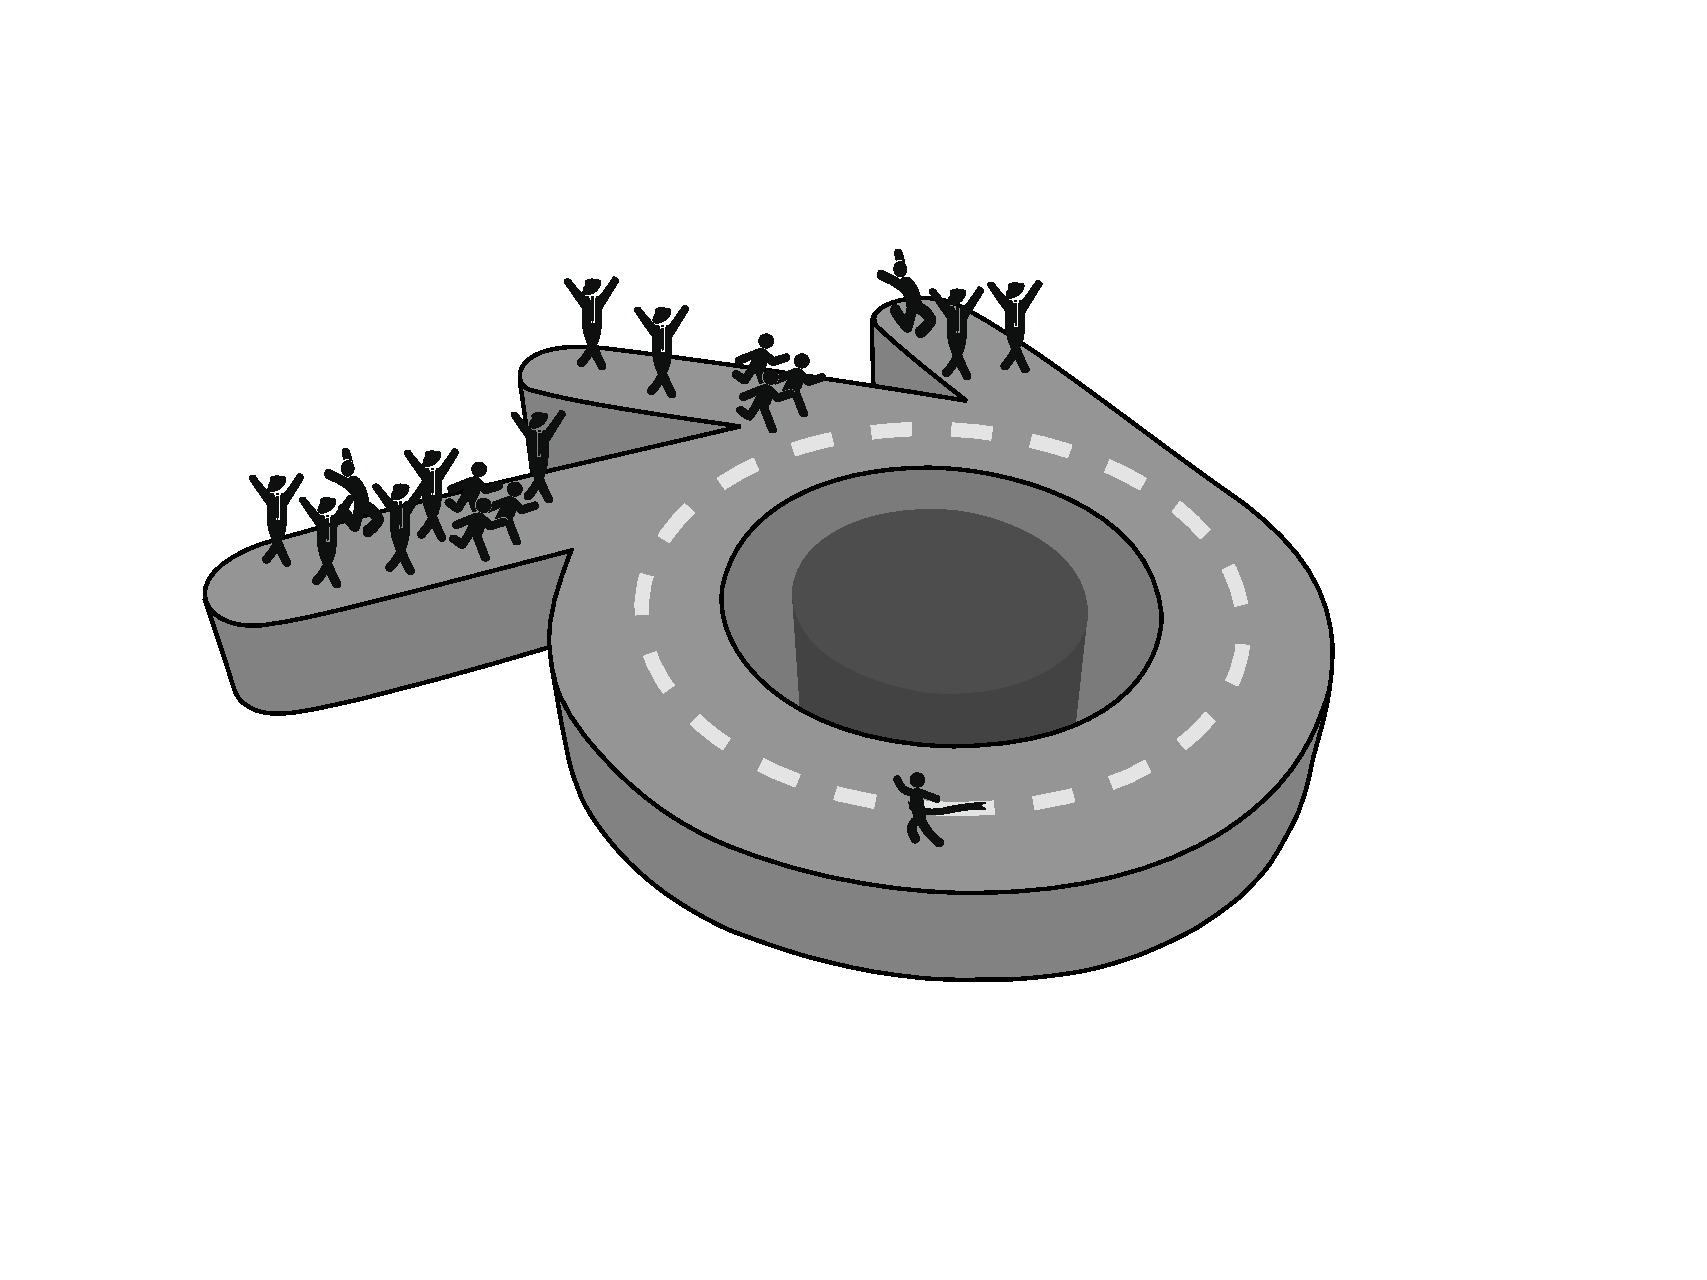
\includegraphics[width=8cm]{logo.pdf}
  \end{center}
\end{figure}
\end{frame}

\maketitle

% black slide for video
\bgroup
\setbeamercolor{background canvas}{bg=black}
\begin{frame}[plain]{}
\end{frame}
\egroup

\begin{frame}{Outline}
  \setbeamertemplate{section in toc}[sections numbered]
  \tableofcontents[hideallsubsections]
\end{frame}

\section{What is Blend'it?}
\begin{frame}{What is Blend'it?}
  Blend'it is a \textbf{Blender plug-in} for \textbf<1>{crowd animation} and \textbf<2>{environment generation}.
  
  \begin{figure}%
\centering
\subfloat{\label{fig:first}\includegraphics<1>[height=6cm]{GUI_map_example.png}} ~ 
\subfloat{\label{fig:second}\includegraphics<1>[height=6cm]{GUI_crowd_example.png}} ~ 
\subfloat{\label{fig:third}\includegraphics<1>[height=6cm]{GUI_simulation_example.png}}
\subfloat{\label{fig:third}\includegraphics<2>[height=5cm]{GUI_env.png}}\\
\label{3figs}

\end{figure}
\end{frame}

\begin{frame}{A Lot of Powerful Software}


\begin{figure}
  \includegraphics<1>[width=.95\textwidth]{golaem.jpg}
  \includegraphics<2>[width=.95\textwidth]{massive.jpg}
  \includegraphics<3>[width=.95\textwidth]{VUE.png}\\
  \only<1>{Golaem}\only<2>{Massive}\only<3>{VUE}
\end{figure}

\end{frame}

\begin{frame}{A Lot of Expensive Software}
  \begin{itemize}
    \item Maya3D: \$1470/year
    \item Golaem: \$5000/year
    \item Massive: \$3,500 - \$16,000/year
    \item VUE: \$1700
    \item Terragen: \$600
  \end{itemize}
\end{frame}

\begin{frame}{Why Blender?}
  Complete open-source 3D software: modelisation, animation, render, ...
    \begin{figure}
        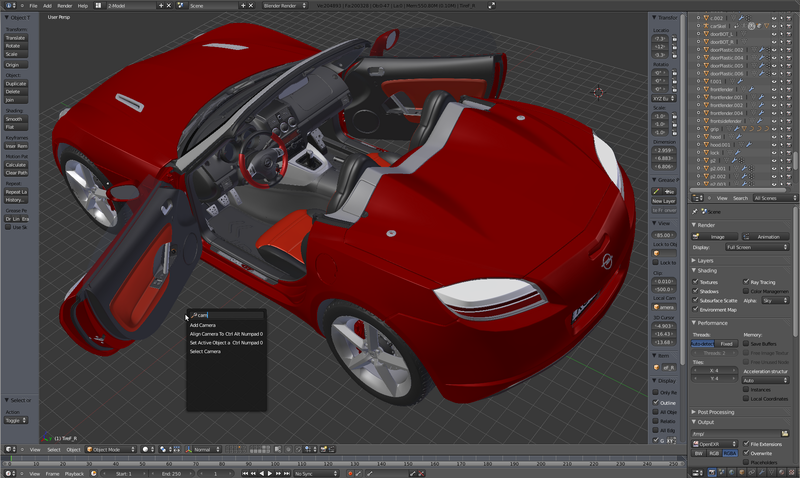
\includegraphics[width=10cm]{blender_mod}
    \end{figure}
\end{frame}

\begin{frame}{Why Blender?}
  Powerful python API (no need to modify the source code of blender)
  \begin{figure}
        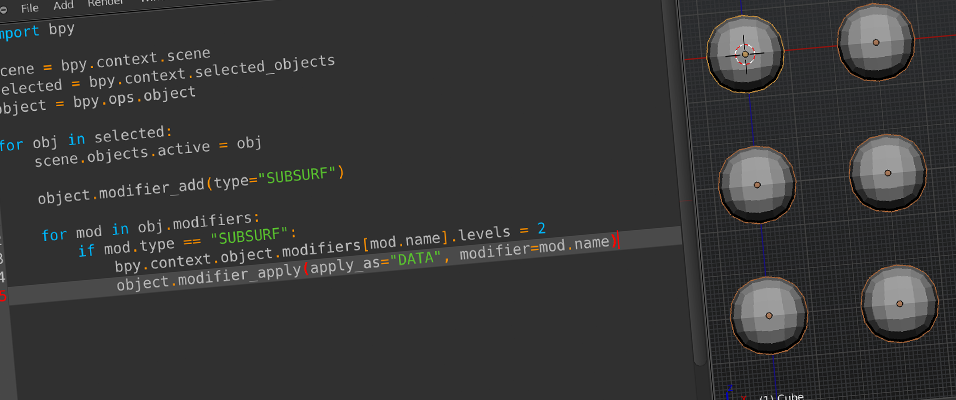
\includegraphics[width=11cm]{blender_script}
    \end{figure}
\end{frame}

\begin{frame}{Project organization}
  \begin{figure}
    \begin{center}
      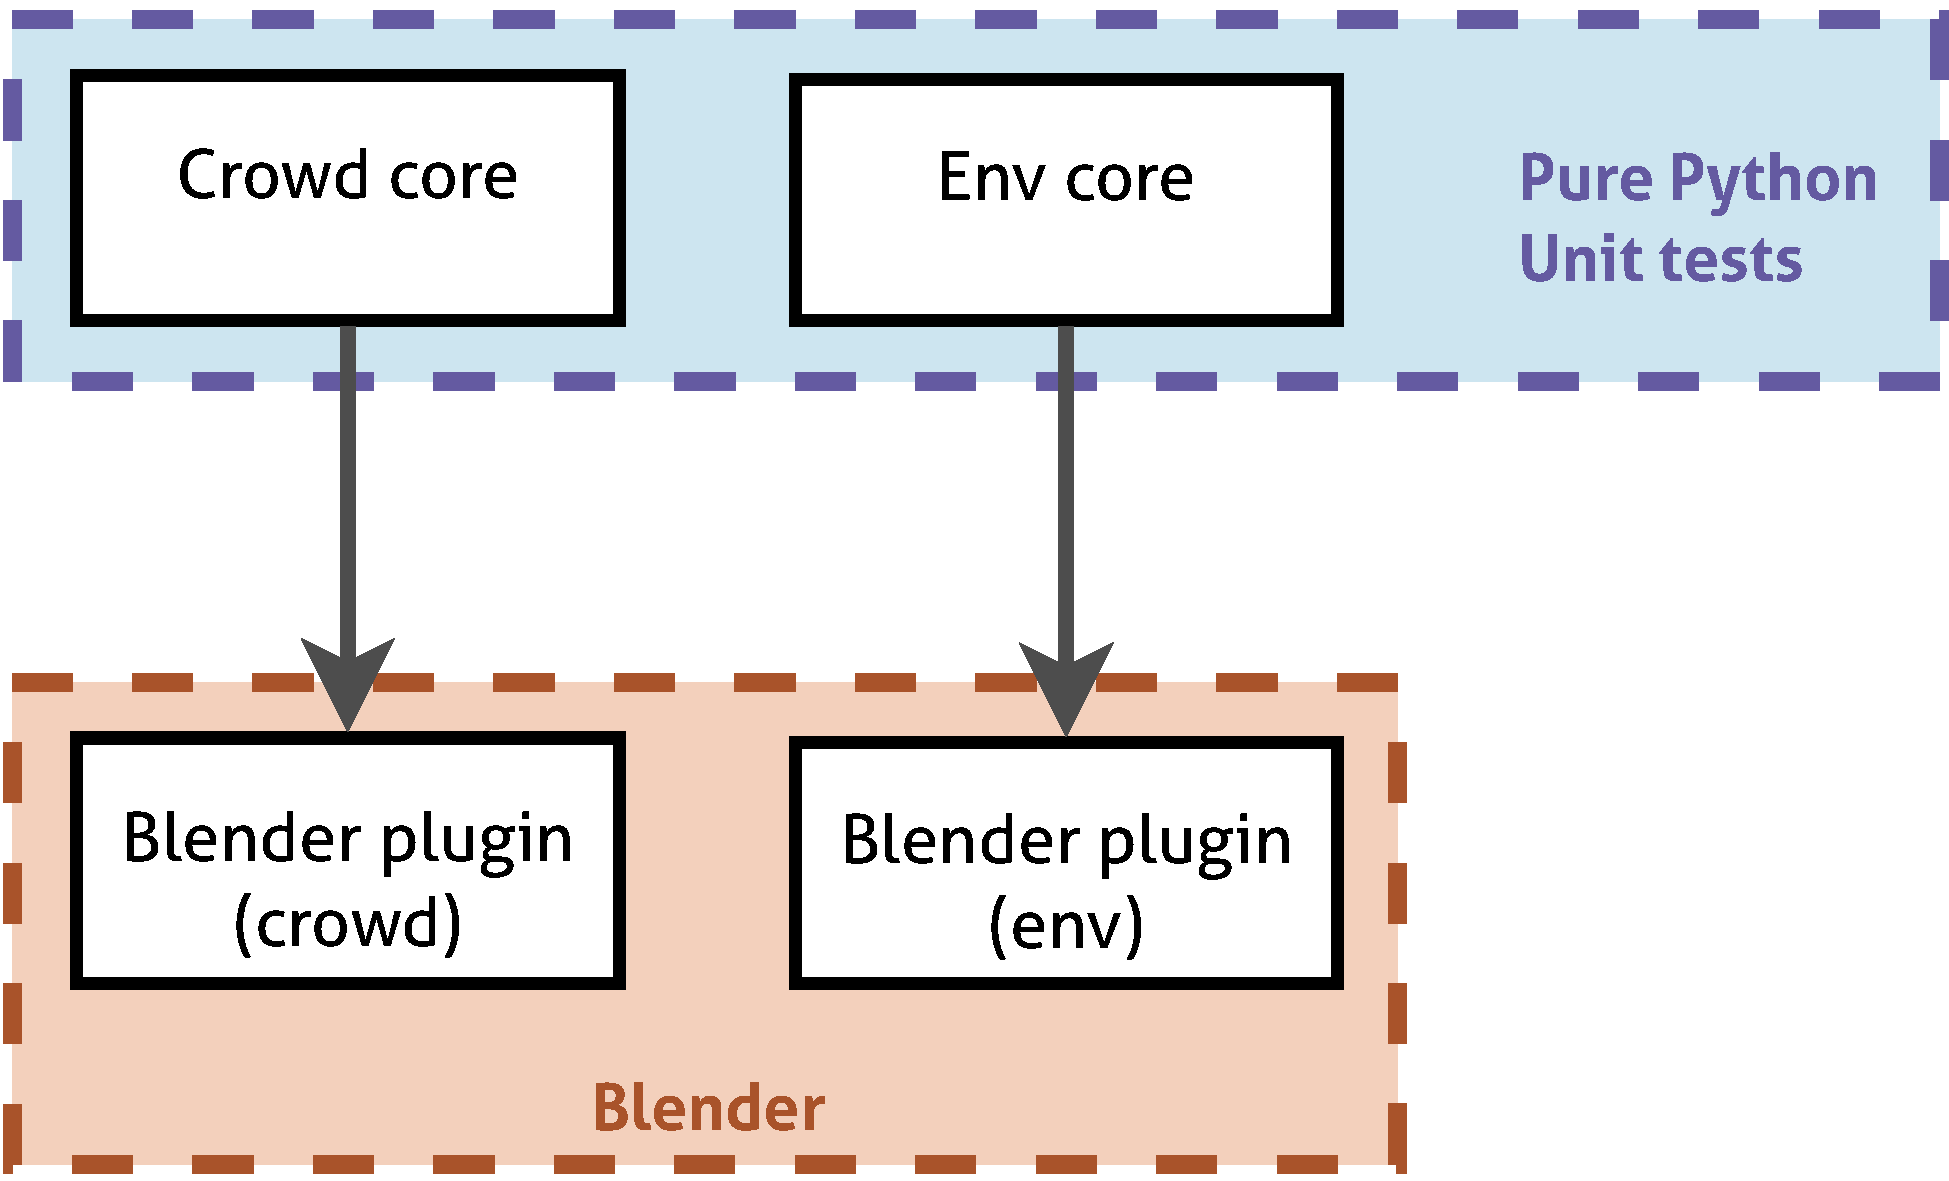
\includegraphics[width=9cm]{orga.pdf}
    \end{center}
  \end{figure}
\end{frame}


\section{Crowd Animation}

\begin{frame}{Crowd Animation - Algorithm}
 	Two approches:
 \begin{itemize}
  \item Automaton based algorithms
  \item Continuous movement
  \begin{itemize}
  \item PLEdestrains: a least-effort approach to crowd simulation
  \item Reciprocal $n$-body collision avoidance
 \end{itemize}
 \end{itemize}
 
\end{frame}

\begin{frame}{Crowd Animation - Algorithm}



\only<1>{
\begin{figure}[h!]
  \centering
  \scalebox{.45}{% Graphic for TeX using PGF
% Title: /home/johanna/Documents/Informatique/M1/Projet/pib/beamer_final/short_path.dia
% Creator: Dia v0.97.3
% CreationDate: Wed Apr 13 17:17:40 2016
% For: johanna
% \usepackage{tikz}
% The following commands are not supported in PSTricks at present
% We define them conditionally, so when they are implemented,
% this pgf file will use them.
\ifx\du\undefined
  \newlength{\du}
\fi
\setlength{\du}{15\unitlength}
\begin{tikzpicture}
\pgftransformxscale{1.000000}
\pgftransformyscale{-1.000000}
\definecolor{dialinecolor}{rgb}{0.000000, 0.000000, 0.000000}
\pgfsetstrokecolor{dialinecolor}
\definecolor{dialinecolor}{rgb}{1.000000, 1.000000, 1.000000}
\pgfsetfillcolor{dialinecolor}
\pgfsetlinewidth{0.200000\du}
\pgfsetdash{}{0pt}
\pgfsetdash{}{0pt}
\pgfsetbuttcap
{
\definecolor{dialinecolor}{rgb}{0.000000, 0.000000, 0.000000}
\pgfsetfillcolor{dialinecolor}
% was here!!!
\definecolor{dialinecolor}{rgb}{0.000000, 0.000000, 0.000000}
\pgfsetstrokecolor{dialinecolor}
\draw (45.000000\du,-13.000000\du)--(75.000000\du,-10.000000\du);
}
\pgfsetlinewidth{0.200000\du}
\pgfsetdash{}{0pt}
\pgfsetdash{}{0pt}
\pgfsetmiterjoin
\pgfsetbuttcap
{
\definecolor{dialinecolor}{rgb}{0.000000, 0.000000, 0.000000}
\pgfsetfillcolor{dialinecolor}
% was here!!!
\definecolor{dialinecolor}{rgb}{0.000000, 0.000000, 0.000000}
\pgfsetstrokecolor{dialinecolor}
\pgfpathmoveto{\pgfpoint{75.000000\du}{-10.000000\du}}
\pgfpathcurveto{\pgfpoint{77.000000\du}{-4.000000\du}}{\pgfpoint{77.000000\du}{6.000000\du}}{\pgfpoint{77.000000\du}{6.000000\du}}
\pgfusepath{stroke}
}
\pgfsetlinewidth{0.200000\du}
\pgfsetdash{}{0pt}
\pgfsetdash{}{0pt}
\pgfsetbuttcap
{
\definecolor{dialinecolor}{rgb}{0.000000, 0.000000, 0.000000}
\pgfsetfillcolor{dialinecolor}
% was here!!!
\definecolor{dialinecolor}{rgb}{0.000000, 0.000000, 0.000000}
\pgfsetstrokecolor{dialinecolor}
\draw (50.000000\du,-7.000000\du)--(70.000000\du,-5.000000\du);
}
\pgfsetlinewidth{0.200000\du}
\pgfsetdash{}{0pt}
\pgfsetdash{}{0pt}
\pgfsetbuttcap
{
\definecolor{dialinecolor}{rgb}{0.000000, 0.000000, 0.000000}
\pgfsetfillcolor{dialinecolor}
% was here!!!
\definecolor{dialinecolor}{rgb}{0.000000, 0.000000, 0.000000}
\pgfsetstrokecolor{dialinecolor}
\draw (70.000000\du,-5.000000\du)--(70.000000\du,2.000000\du);
}
\pgfsetlinewidth{0.200000\du}
\pgfsetdash{}{0pt}
\pgfsetdash{}{0pt}
\pgfsetmiterjoin
\pgfsetbuttcap
{
\definecolor{dialinecolor}{rgb}{0.000000, 0.000000, 0.000000}
\pgfsetfillcolor{dialinecolor}
% was here!!!
\definecolor{dialinecolor}{rgb}{0.000000, 0.000000, 0.000000}
\pgfsetstrokecolor{dialinecolor}
\pgfpathmoveto{\pgfpoint{50.000000\du}{-7.000000\du}}
\pgfpathcurveto{\pgfpoint{50.000000\du}{2.000000\du}}{\pgfpoint{67.676000\du}{2.000000\du}}{\pgfpoint{70.000000\du}{2.000000\du}}
\pgfusepath{stroke}
}
\pgfsetlinewidth{0.200000\du}
\pgfsetdash{}{0pt}
\pgfsetdash{}{0pt}
\pgfsetbuttcap
\pgfsetmiterjoin
\pgfsetlinewidth{0.200000\du}
\pgfsetbuttcap
\pgfsetmiterjoin
\pgfsetdash{}{0pt}
\definecolor{dialinecolor}{rgb}{1.000000, 1.000000, 1.000000}
\pgfsetfillcolor{dialinecolor}
\fill (72.000000\du,-7.000000\du)--(72.750000\du,-7.250000\du)--(73.000000\du,-8.000000\du)--(73.250000\du,-7.250000\du)--(74.000000\du,-7.000000\du)--(73.250000\du,-6.750000\du)--(73.000000\du,-6.000000\du)--(72.750000\du,-6.750000\du)--cycle;
\definecolor{dialinecolor}{rgb}{0.000000, 0.000000, 0.000000}
\pgfsetstrokecolor{dialinecolor}
\draw (72.000000\du,-7.000000\du)--(72.750000\du,-7.250000\du)--(73.000000\du,-8.000000\du)--(73.250000\du,-7.250000\du)--(74.000000\du,-7.000000\du)--(73.250000\du,-6.750000\du)--(73.000000\du,-6.000000\du)--(72.750000\du,-6.750000\du)--cycle;
\pgfsetbuttcap
\pgfsetmiterjoin
\pgfsetdash{}{0pt}
\definecolor{dialinecolor}{rgb}{0.000000, 0.000000, 0.000000}
\pgfsetstrokecolor{dialinecolor}
\draw (72.000000\du,-7.000000\du)--(72.750000\du,-7.250000\du)--(73.000000\du,-8.000000\du)--(73.250000\du,-7.250000\du)--(74.000000\du,-7.000000\du)--(73.250000\du,-6.750000\du)--(73.000000\du,-6.000000\du)--(72.750000\du,-6.750000\du)--cycle;
\pgfsetlinewidth{0.200000\du}
\pgfsetdash{}{0pt}
\pgfsetdash{}{0pt}
\pgfsetbuttcap
\pgfsetmiterjoin
\pgfsetlinewidth{0.200000\du}
\pgfsetbuttcap
\pgfsetmiterjoin
\pgfsetdash{}{0pt}
\definecolor{dialinecolor}{rgb}{1.000000, 1.000000, 1.000000}
\pgfsetfillcolor{dialinecolor}
\fill (47.500000\du,-10.499997\du)--(48.000000\du,-9.499997\du)--(47.000000\du,-9.499997\du)--cycle;
\definecolor{dialinecolor}{rgb}{1.000000, 0.027451, 0.027451}
\pgfsetstrokecolor{dialinecolor}
\draw (47.500000\du,-10.499997\du)--(48.000000\du,-9.499997\du)--(47.000000\du,-9.499997\du)--cycle;
\pgfsetlinewidth{0.200000\du}
\pgfsetdash{}{0pt}
\pgfsetdash{}{0pt}
\pgfsetbuttcap
\pgfsetmiterjoin
\pgfsetlinewidth{0.200000\du}
\pgfsetbuttcap
\pgfsetmiterjoin
\pgfsetdash{}{0pt}
\definecolor{dialinecolor}{rgb}{1.000000, 1.000000, 1.000000}
\pgfsetfillcolor{dialinecolor}
\fill (56.500000\du,-8.000000\du)--(57.000000\du,-7.000000\du)--(56.000000\du,-7.000000\du)--cycle;
\definecolor{dialinecolor}{rgb}{0.000000, 0.000000, 0.000000}
\pgfsetstrokecolor{dialinecolor}
\draw (56.500000\du,-8.000000\du)--(57.000000\du,-7.000000\du)--(56.000000\du,-7.000000\du)--cycle;
\pgfsetlinewidth{0.200000\du}
\pgfsetdash{}{0pt}
\pgfsetdash{}{0pt}
\pgfsetbuttcap
\pgfsetmiterjoin
\pgfsetlinewidth{0.200000\du}
\pgfsetbuttcap
\pgfsetmiterjoin
\pgfsetdash{}{0pt}
\definecolor{dialinecolor}{rgb}{1.000000, 1.000000, 1.000000}
\pgfsetfillcolor{dialinecolor}
\fill (56.500000\du,-11.000000\du)--(57.000000\du,-10.000000\du)--(56.000000\du,-10.000000\du)--cycle;
\definecolor{dialinecolor}{rgb}{0.000000, 0.000000, 0.000000}
\pgfsetstrokecolor{dialinecolor}
\draw (56.500000\du,-11.000000\du)--(57.000000\du,-10.000000\du)--(56.000000\du,-10.000000\du)--cycle;
\pgfsetlinewidth{0.200000\du}
\pgfsetdash{}{0pt}
\pgfsetdash{}{0pt}
\pgfsetbuttcap
\pgfsetmiterjoin
\pgfsetlinewidth{0.200000\du}
\pgfsetbuttcap
\pgfsetmiterjoin
\pgfsetdash{}{0pt}
\definecolor{dialinecolor}{rgb}{1.000000, 1.000000, 1.000000}
\pgfsetfillcolor{dialinecolor}
\fill (59.500000\du,-11.000000\du)--(60.000000\du,-10.000000\du)--(59.000000\du,-10.000000\du)--cycle;
\definecolor{dialinecolor}{rgb}{0.000000, 0.000000, 0.000000}
\pgfsetstrokecolor{dialinecolor}
\draw (59.500000\du,-11.000000\du)--(60.000000\du,-10.000000\du)--(59.000000\du,-10.000000\du)--cycle;
\pgfsetlinewidth{0.200000\du}
\pgfsetdash{}{0pt}
\pgfsetdash{}{0pt}
\pgfsetbuttcap
\pgfsetmiterjoin
\pgfsetlinewidth{0.200000\du}
\pgfsetbuttcap
\pgfsetmiterjoin
\pgfsetdash{}{0pt}
\definecolor{dialinecolor}{rgb}{1.000000, 1.000000, 1.000000}
\pgfsetfillcolor{dialinecolor}
\fill (59.500000\du,-8.000000\du)--(60.000000\du,-7.000000\du)--(59.000000\du,-7.000000\du)--cycle;
\definecolor{dialinecolor}{rgb}{0.000000, 0.000000, 0.000000}
\pgfsetstrokecolor{dialinecolor}
\draw (59.500000\du,-8.000000\du)--(60.000000\du,-7.000000\du)--(59.000000\du,-7.000000\du)--cycle;
\pgfsetlinewidth{0.200000\du}
\pgfsetdash{}{0pt}
\pgfsetdash{}{0pt}
\pgfsetbuttcap
\pgfsetmiterjoin
\pgfsetlinewidth{0.200000\du}
\pgfsetbuttcap
\pgfsetmiterjoin
\pgfsetdash{}{0pt}
\definecolor{dialinecolor}{rgb}{1.000000, 1.000000, 1.000000}
\pgfsetfillcolor{dialinecolor}
\fill (62.500000\du,-10.000000\du)--(63.000000\du,-9.000000\du)--(62.000000\du,-9.000000\du)--cycle;
\definecolor{dialinecolor}{rgb}{0.000000, 0.000000, 0.000000}
\pgfsetstrokecolor{dialinecolor}
\draw (62.500000\du,-10.000000\du)--(63.000000\du,-9.000000\du)--(62.000000\du,-9.000000\du)--cycle;
\pgfsetlinewidth{0.200000\du}
\pgfsetdash{}{0pt}
\pgfsetdash{}{0pt}
\pgfsetbuttcap
\pgfsetmiterjoin
\pgfsetlinewidth{0.200000\du}
\pgfsetbuttcap
\pgfsetmiterjoin
\pgfsetdash{}{0pt}
\definecolor{dialinecolor}{rgb}{1.000000, 1.000000, 1.000000}
\pgfsetfillcolor{dialinecolor}
\fill (62.500000\du,-7.000000\du)--(63.000000\du,-6.000000\du)--(62.000000\du,-6.000000\du)--cycle;
\definecolor{dialinecolor}{rgb}{0.000000, 0.000000, 0.000000}
\pgfsetstrokecolor{dialinecolor}
\draw (62.500000\du,-7.000000\du)--(63.000000\du,-6.000000\du)--(62.000000\du,-6.000000\du)--cycle;
\pgfsetlinewidth{0.200000\du}
\pgfsetdash{}{0pt}
\pgfsetdash{}{0pt}
\pgfsetbuttcap
\pgfsetmiterjoin
\pgfsetlinewidth{0.200000\du}
\pgfsetbuttcap
\pgfsetmiterjoin
\pgfsetdash{}{0pt}
\definecolor{dialinecolor}{rgb}{1.000000, 1.000000, 1.000000}
\pgfsetfillcolor{dialinecolor}
\fill (65.500000\du,-10.000000\du)--(66.000000\du,-9.000000\du)--(65.000000\du,-9.000000\du)--cycle;
\definecolor{dialinecolor}{rgb}{0.000000, 0.000000, 0.000000}
\pgfsetstrokecolor{dialinecolor}
\draw (65.500000\du,-10.000000\du)--(66.000000\du,-9.000000\du)--(65.000000\du,-9.000000\du)--cycle;
\pgfsetlinewidth{0.200000\du}
\pgfsetdash{}{0pt}
\pgfsetdash{}{0pt}
\pgfsetbuttcap
\pgfsetmiterjoin
\pgfsetlinewidth{0.200000\du}
\pgfsetbuttcap
\pgfsetmiterjoin
\pgfsetdash{}{0pt}
\definecolor{dialinecolor}{rgb}{1.000000, 1.000000, 1.000000}
\pgfsetfillcolor{dialinecolor}
\fill (64.500000\du,-7.000000\du)--(65.000000\du,-6.000000\du)--(64.000000\du,-6.000000\du)--cycle;
\definecolor{dialinecolor}{rgb}{0.000000, 0.000000, 0.000000}
\pgfsetstrokecolor{dialinecolor}
\draw (64.500000\du,-7.000000\du)--(65.000000\du,-6.000000\du)--(64.000000\du,-6.000000\du)--cycle;
\pgfsetlinewidth{0.200000\du}
\pgfsetdash{}{0pt}
\pgfsetdash{}{0pt}
\pgfsetbuttcap
\pgfsetmiterjoin
\pgfsetlinewidth{0.200000\du}
\pgfsetbuttcap
\pgfsetmiterjoin
\pgfsetdash{}{0pt}
\definecolor{dialinecolor}{rgb}{1.000000, 1.000000, 1.000000}
\pgfsetfillcolor{dialinecolor}
\fill (61.500000\du,-11.000000\du)--(62.000000\du,-10.000000\du)--(61.000000\du,-10.000000\du)--cycle;
\definecolor{dialinecolor}{rgb}{0.000000, 0.000000, 0.000000}
\pgfsetstrokecolor{dialinecolor}
\draw (61.500000\du,-11.000000\du)--(62.000000\du,-10.000000\du)--(61.000000\du,-10.000000\du)--cycle;
\end{tikzpicture}
}
  %\caption{}\label{}
\end{figure}
}

\only<2>{
\begin{figure}[h!]
  \centering
  \scalebox{.45}{% Graphic for TeX using PGF
% Title: /home/johanna/Documents/Informatique/M1/Projet/pib/beamer_final/short_path_grid.dia
% Creator: Dia v0.97.3
% CreationDate: Wed Apr 13 20:23:16 2016
% For: johanna
% \usepackage{tikz}
% The following commands are not supported in PSTricks at present
% We define them conditionally, so when they are implemented,
% this pgf file will use them.
\ifx\du\undefined
  \newlength{\du}
\fi
\setlength{\du}{15\unitlength}
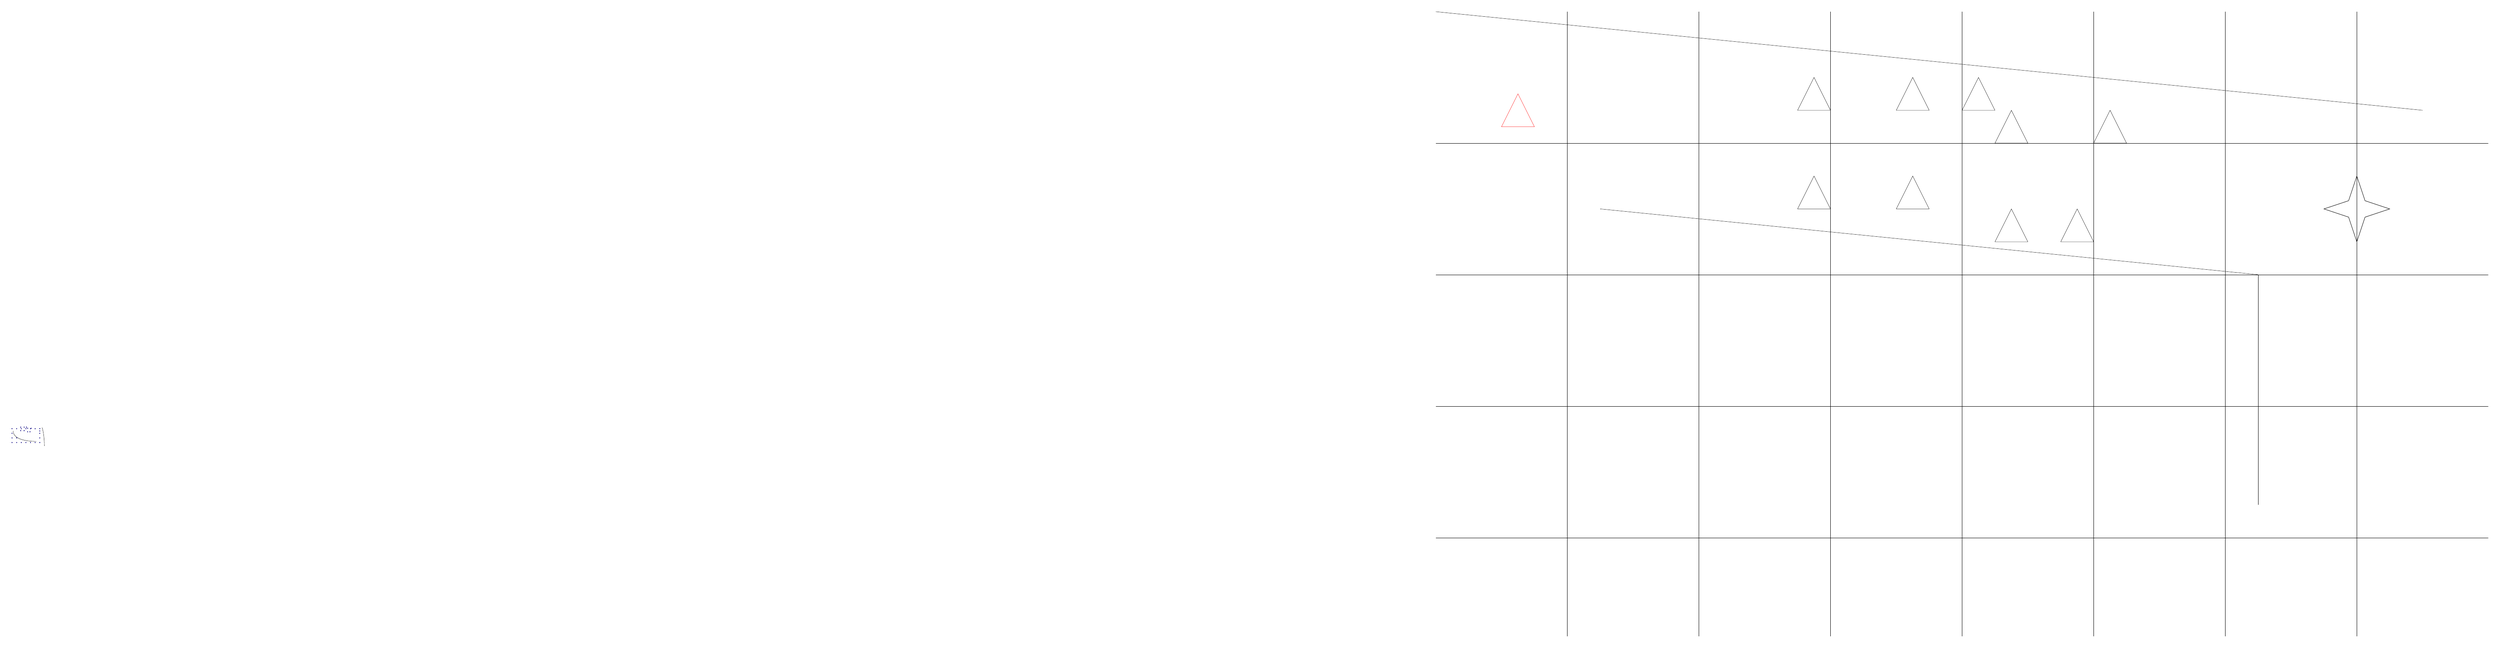
\begin{tikzpicture}
\pgftransformxscale{1.000000}
\pgftransformyscale{-1.000000}
\definecolor{dialinecolor}{rgb}{0.000000, 0.000000, 0.000000}
\pgfsetstrokecolor{dialinecolor}
\definecolor{dialinecolor}{rgb}{1.000000, 1.000000, 1.000000}
\pgfsetfillcolor{dialinecolor}
\pgfsetlinewidth{0.200000\du}
\pgfsetdash{}{0pt}
\pgfsetdash{}{0pt}
\pgfsetbuttcap
{
\definecolor{dialinecolor}{rgb}{0.000000, 0.000000, 0.000000}
\pgfsetfillcolor{dialinecolor}
% was here!!!
\definecolor{dialinecolor}{rgb}{0.000000, 0.000000, 0.000000}
\pgfsetstrokecolor{dialinecolor}
\draw (45.000000\du,-13.000000\du)--(75.000000\du,-10.000000\du);
}
\pgfsetlinewidth{0.200000\du}
\pgfsetdash{}{0pt}
\pgfsetdash{}{0pt}
\pgfsetmiterjoin
\pgfsetbuttcap
{
\definecolor{dialinecolor}{rgb}{0.000000, 0.000000, 0.000000}
\pgfsetfillcolor{dialinecolor}
% was here!!!
\definecolor{dialinecolor}{rgb}{0.000000, 0.000000, 0.000000}
\pgfsetstrokecolor{dialinecolor}
\pgfpathmoveto{\pgfpoint{75.000000\du}{-10.000000\du}}
\pgfpathcurveto{\pgfpoint{77.000000\du}{-4.000000\du}}{\pgfpoint{77.000000\du}{6.000000\du}}{\pgfpoint{77.000000\du}{6.000000\du}}
\pgfusepath{stroke}
}
\pgfsetlinewidth{0.200000\du}
\pgfsetdash{}{0pt}
\pgfsetdash{}{0pt}
\pgfsetbuttcap
{
\definecolor{dialinecolor}{rgb}{0.000000, 0.000000, 0.000000}
\pgfsetfillcolor{dialinecolor}
% was here!!!
\definecolor{dialinecolor}{rgb}{0.000000, 0.000000, 0.000000}
\pgfsetstrokecolor{dialinecolor}
\draw (50.000000\du,-7.000000\du)--(70.000000\du,-5.000000\du);
}
\pgfsetlinewidth{0.200000\du}
\pgfsetdash{}{0pt}
\pgfsetdash{}{0pt}
\pgfsetbuttcap
{
\definecolor{dialinecolor}{rgb}{0.000000, 0.000000, 0.000000}
\pgfsetfillcolor{dialinecolor}
% was here!!!
\definecolor{dialinecolor}{rgb}{0.000000, 0.000000, 0.000000}
\pgfsetstrokecolor{dialinecolor}
\draw (70.000000\du,-5.000000\du)--(70.000000\du,2.000000\du);
}
\pgfsetlinewidth{0.200000\du}
\pgfsetdash{}{0pt}
\pgfsetdash{}{0pt}
\pgfsetmiterjoin
\pgfsetbuttcap
{
\definecolor{dialinecolor}{rgb}{0.000000, 0.000000, 0.000000}
\pgfsetfillcolor{dialinecolor}
% was here!!!
\definecolor{dialinecolor}{rgb}{0.000000, 0.000000, 0.000000}
\pgfsetstrokecolor{dialinecolor}
\pgfpathmoveto{\pgfpoint{50.000000\du}{-7.000000\du}}
\pgfpathcurveto{\pgfpoint{50.000000\du}{2.000000\du}}{\pgfpoint{67.676000\du}{2.000000\du}}{\pgfpoint{70.000000\du}{2.000000\du}}
\pgfusepath{stroke}
}
\pgfsetlinewidth{0.200000\du}
\pgfsetdash{}{0pt}
\pgfsetdash{}{0pt}
\pgfsetbuttcap
\pgfsetmiterjoin
\pgfsetlinewidth{0.200000\du}
\pgfsetbuttcap
\pgfsetmiterjoin
\pgfsetdash{}{0pt}
\definecolor{dialinecolor}{rgb}{1.000000, 1.000000, 1.000000}
\pgfsetfillcolor{dialinecolor}
\fill (72.000000\du,-7.000000\du)--(72.750000\du,-7.250000\du)--(73.000000\du,-8.000000\du)--(73.250000\du,-7.250000\du)--(74.000000\du,-7.000000\du)--(73.250000\du,-6.750000\du)--(73.000000\du,-6.000000\du)--(72.750000\du,-6.750000\du)--cycle;
\definecolor{dialinecolor}{rgb}{0.000000, 0.000000, 0.000000}
\pgfsetstrokecolor{dialinecolor}
\draw (72.000000\du,-7.000000\du)--(72.750000\du,-7.250000\du)--(73.000000\du,-8.000000\du)--(73.250000\du,-7.250000\du)--(74.000000\du,-7.000000\du)--(73.250000\du,-6.750000\du)--(73.000000\du,-6.000000\du)--(72.750000\du,-6.750000\du)--cycle;
\pgfsetbuttcap
\pgfsetmiterjoin
\pgfsetdash{}{0pt}
\definecolor{dialinecolor}{rgb}{0.000000, 0.000000, 0.000000}
\pgfsetstrokecolor{dialinecolor}
\draw (72.000000\du,-7.000000\du)--(72.750000\du,-7.250000\du)--(73.000000\du,-8.000000\du)--(73.250000\du,-7.250000\du)--(74.000000\du,-7.000000\du)--(73.250000\du,-6.750000\du)--(73.000000\du,-6.000000\du)--(72.750000\du,-6.750000\du)--cycle;
\pgfsetlinewidth{0.200000\du}
\pgfsetdash{}{0pt}
\pgfsetdash{}{0pt}
\pgfsetbuttcap
\pgfsetmiterjoin
\pgfsetlinewidth{0.200000\du}
\pgfsetbuttcap
\pgfsetmiterjoin
\pgfsetdash{}{0pt}
\definecolor{dialinecolor}{rgb}{1.000000, 1.000000, 1.000000}
\pgfsetfillcolor{dialinecolor}
\fill (47.500000\du,-10.500000\du)--(48.000000\du,-9.500000\du)--(47.000000\du,-9.500000\du)--cycle;
\definecolor{dialinecolor}{rgb}{1.000000, 0.027451, 0.027451}
\pgfsetstrokecolor{dialinecolor}
\draw (47.500000\du,-10.500000\du)--(48.000000\du,-9.500000\du)--(47.000000\du,-9.500000\du)--cycle;
\pgfsetlinewidth{0.200000\du}
\pgfsetdash{}{0pt}
\pgfsetdash{}{0pt}
\pgfsetbuttcap
\pgfsetmiterjoin
\pgfsetlinewidth{0.200000\du}
\pgfsetbuttcap
\pgfsetmiterjoin
\pgfsetdash{}{0pt}
\definecolor{dialinecolor}{rgb}{1.000000, 1.000000, 1.000000}
\pgfsetfillcolor{dialinecolor}
\fill (56.500000\du,-8.000000\du)--(57.000000\du,-7.000000\du)--(56.000000\du,-7.000000\du)--cycle;
\definecolor{dialinecolor}{rgb}{0.000000, 0.000000, 0.000000}
\pgfsetstrokecolor{dialinecolor}
\draw (56.500000\du,-8.000000\du)--(57.000000\du,-7.000000\du)--(56.000000\du,-7.000000\du)--cycle;
\pgfsetlinewidth{0.200000\du}
\pgfsetdash{}{0pt}
\pgfsetdash{}{0pt}
\pgfsetbuttcap
\pgfsetmiterjoin
\pgfsetlinewidth{0.200000\du}
\pgfsetbuttcap
\pgfsetmiterjoin
\pgfsetdash{}{0pt}
\definecolor{dialinecolor}{rgb}{1.000000, 1.000000, 1.000000}
\pgfsetfillcolor{dialinecolor}
\fill (56.500000\du,-11.000000\du)--(57.000000\du,-10.000000\du)--(56.000000\du,-10.000000\du)--cycle;
\definecolor{dialinecolor}{rgb}{0.000000, 0.000000, 0.000000}
\pgfsetstrokecolor{dialinecolor}
\draw (56.500000\du,-11.000000\du)--(57.000000\du,-10.000000\du)--(56.000000\du,-10.000000\du)--cycle;
\pgfsetlinewidth{0.200000\du}
\pgfsetdash{}{0pt}
\pgfsetdash{}{0pt}
\pgfsetbuttcap
\pgfsetmiterjoin
\pgfsetlinewidth{0.200000\du}
\pgfsetbuttcap
\pgfsetmiterjoin
\pgfsetdash{}{0pt}
\definecolor{dialinecolor}{rgb}{1.000000, 1.000000, 1.000000}
\pgfsetfillcolor{dialinecolor}
\fill (59.500000\du,-11.000000\du)--(60.000000\du,-10.000000\du)--(59.000000\du,-10.000000\du)--cycle;
\definecolor{dialinecolor}{rgb}{0.000000, 0.000000, 0.000000}
\pgfsetstrokecolor{dialinecolor}
\draw (59.500000\du,-11.000000\du)--(60.000000\du,-10.000000\du)--(59.000000\du,-10.000000\du)--cycle;
\pgfsetlinewidth{0.200000\du}
\pgfsetdash{}{0pt}
\pgfsetdash{}{0pt}
\pgfsetbuttcap
\pgfsetmiterjoin
\pgfsetlinewidth{0.200000\du}
\pgfsetbuttcap
\pgfsetmiterjoin
\pgfsetdash{}{0pt}
\definecolor{dialinecolor}{rgb}{1.000000, 1.000000, 1.000000}
\pgfsetfillcolor{dialinecolor}
\fill (59.500000\du,-8.000000\du)--(60.000000\du,-7.000000\du)--(59.000000\du,-7.000000\du)--cycle;
\definecolor{dialinecolor}{rgb}{0.000000, 0.000000, 0.000000}
\pgfsetstrokecolor{dialinecolor}
\draw (59.500000\du,-8.000000\du)--(60.000000\du,-7.000000\du)--(59.000000\du,-7.000000\du)--cycle;
\pgfsetlinewidth{0.200000\du}
\pgfsetdash{}{0pt}
\pgfsetdash{}{0pt}
\pgfsetbuttcap
\pgfsetmiterjoin
\pgfsetlinewidth{0.200000\du}
\pgfsetbuttcap
\pgfsetmiterjoin
\pgfsetdash{}{0pt}
\definecolor{dialinecolor}{rgb}{1.000000, 1.000000, 1.000000}
\pgfsetfillcolor{dialinecolor}
\fill (62.500000\du,-10.000000\du)--(63.000000\du,-9.000000\du)--(62.000000\du,-9.000000\du)--cycle;
\definecolor{dialinecolor}{rgb}{0.000000, 0.000000, 0.000000}
\pgfsetstrokecolor{dialinecolor}
\draw (62.500000\du,-10.000000\du)--(63.000000\du,-9.000000\du)--(62.000000\du,-9.000000\du)--cycle;
\pgfsetlinewidth{0.200000\du}
\pgfsetdash{}{0pt}
\pgfsetdash{}{0pt}
\pgfsetbuttcap
\pgfsetmiterjoin
\pgfsetlinewidth{0.200000\du}
\pgfsetbuttcap
\pgfsetmiterjoin
\pgfsetdash{}{0pt}
\definecolor{dialinecolor}{rgb}{1.000000, 1.000000, 1.000000}
\pgfsetfillcolor{dialinecolor}
\fill (62.500000\du,-7.000000\du)--(63.000000\du,-6.000000\du)--(62.000000\du,-6.000000\du)--cycle;
\definecolor{dialinecolor}{rgb}{0.000000, 0.000000, 0.000000}
\pgfsetstrokecolor{dialinecolor}
\draw (62.500000\du,-7.000000\du)--(63.000000\du,-6.000000\du)--(62.000000\du,-6.000000\du)--cycle;
\pgfsetlinewidth{0.200000\du}
\pgfsetdash{}{0pt}
\pgfsetdash{}{0pt}
\pgfsetbuttcap
\pgfsetmiterjoin
\pgfsetlinewidth{0.200000\du}
\pgfsetbuttcap
\pgfsetmiterjoin
\pgfsetdash{}{0pt}
\definecolor{dialinecolor}{rgb}{1.000000, 1.000000, 1.000000}
\pgfsetfillcolor{dialinecolor}
\fill (65.500000\du,-10.000000\du)--(66.000000\du,-9.000000\du)--(65.000000\du,-9.000000\du)--cycle;
\definecolor{dialinecolor}{rgb}{0.000000, 0.000000, 0.000000}
\pgfsetstrokecolor{dialinecolor}
\draw (65.500000\du,-10.000000\du)--(66.000000\du,-9.000000\du)--(65.000000\du,-9.000000\du)--cycle;
\pgfsetlinewidth{0.200000\du}
\pgfsetdash{}{0pt}
\pgfsetdash{}{0pt}
\pgfsetbuttcap
\pgfsetmiterjoin
\pgfsetlinewidth{0.200000\du}
\pgfsetbuttcap
\pgfsetmiterjoin
\pgfsetdash{}{0pt}
\definecolor{dialinecolor}{rgb}{1.000000, 1.000000, 1.000000}
\pgfsetfillcolor{dialinecolor}
\fill (64.500000\du,-7.000000\du)--(65.000000\du,-6.000000\du)--(64.000000\du,-6.000000\du)--cycle;
\definecolor{dialinecolor}{rgb}{0.000000, 0.000000, 0.000000}
\pgfsetstrokecolor{dialinecolor}
\draw (64.500000\du,-7.000000\du)--(65.000000\du,-6.000000\du)--(64.000000\du,-6.000000\du)--cycle;
\pgfsetlinewidth{0.200000\du}
\pgfsetdash{}{0pt}
\pgfsetdash{}{0pt}
\pgfsetbuttcap
\pgfsetmiterjoin
\pgfsetlinewidth{0.200000\du}
\pgfsetbuttcap
\pgfsetmiterjoin
\pgfsetdash{}{0pt}
\definecolor{dialinecolor}{rgb}{1.000000, 1.000000, 1.000000}
\pgfsetfillcolor{dialinecolor}
\fill (61.500000\du,-11.000000\du)--(62.000000\du,-10.000000\du)--(61.000000\du,-10.000000\du)--cycle;
\definecolor{dialinecolor}{rgb}{0.000000, 0.000000, 0.000000}
\pgfsetstrokecolor{dialinecolor}
\draw (61.500000\du,-11.000000\du)--(62.000000\du,-10.000000\du)--(61.000000\du,-10.000000\du)--cycle;
\pgfsetlinewidth{0.100000\du}
\pgfsetdash{}{0pt}
\pgfsetdash{}{0pt}
\pgfsetbuttcap
{
\definecolor{dialinecolor}{rgb}{0.000000, 0.000000, 0.000000}
\pgfsetfillcolor{dialinecolor}
% was here!!!
\definecolor{dialinecolor}{rgb}{0.000000, 0.000000, 0.000000}
\pgfsetstrokecolor{dialinecolor}
\draw (49.000000\du,-13.000000\du)--(49.000000\du,6.000000\du);
}
\pgfsetlinewidth{0.100000\du}
\pgfsetdash{}{0pt}
\pgfsetdash{}{0pt}
\pgfsetbuttcap
{
\definecolor{dialinecolor}{rgb}{0.000000, 0.000000, 0.000000}
\pgfsetfillcolor{dialinecolor}
% was here!!!
\definecolor{dialinecolor}{rgb}{0.000000, 0.000000, 0.000000}
\pgfsetstrokecolor{dialinecolor}
\draw (53.000000\du,-13.000000\du)--(53.000000\du,6.000000\du);
}
\pgfsetlinewidth{0.100000\du}
\pgfsetdash{}{0pt}
\pgfsetdash{}{0pt}
\pgfsetbuttcap
{
\definecolor{dialinecolor}{rgb}{0.000000, 0.000000, 0.000000}
\pgfsetfillcolor{dialinecolor}
% was here!!!
\definecolor{dialinecolor}{rgb}{0.000000, 0.000000, 0.000000}
\pgfsetstrokecolor{dialinecolor}
\draw (57.000000\du,-13.000000\du)--(57.000000\du,6.000000\du);
}
\pgfsetlinewidth{0.100000\du}
\pgfsetdash{}{0pt}
\pgfsetdash{}{0pt}
\pgfsetbuttcap
{
\definecolor{dialinecolor}{rgb}{0.000000, 0.000000, 0.000000}
\pgfsetfillcolor{dialinecolor}
% was here!!!
\definecolor{dialinecolor}{rgb}{0.000000, 0.000000, 0.000000}
\pgfsetstrokecolor{dialinecolor}
\draw (61.000000\du,-13.000000\du)--(61.000000\du,6.000000\du);
}
\pgfsetlinewidth{0.100000\du}
\pgfsetdash{}{0pt}
\pgfsetdash{}{0pt}
\pgfsetbuttcap
{
\definecolor{dialinecolor}{rgb}{0.000000, 0.000000, 0.000000}
\pgfsetfillcolor{dialinecolor}
% was here!!!
\definecolor{dialinecolor}{rgb}{0.000000, 0.000000, 0.000000}
\pgfsetstrokecolor{dialinecolor}
\draw (65.000000\du,-13.000000\du)--(65.000000\du,6.000000\du);
}
\pgfsetlinewidth{0.100000\du}
\pgfsetdash{}{0pt}
\pgfsetdash{}{0pt}
\pgfsetbuttcap
{
\definecolor{dialinecolor}{rgb}{0.000000, 0.000000, 0.000000}
\pgfsetfillcolor{dialinecolor}
% was here!!!
\definecolor{dialinecolor}{rgb}{0.000000, 0.000000, 0.000000}
\pgfsetstrokecolor{dialinecolor}
\draw (69.000000\du,-13.000000\du)--(69.000000\du,6.000000\du);
}
\pgfsetlinewidth{0.100000\du}
\pgfsetdash{}{0pt}
\pgfsetdash{}{0pt}
\pgfsetbuttcap
{
\definecolor{dialinecolor}{rgb}{0.000000, 0.000000, 0.000000}
\pgfsetfillcolor{dialinecolor}
% was here!!!
\definecolor{dialinecolor}{rgb}{0.000000, 0.000000, 0.000000}
\pgfsetstrokecolor{dialinecolor}
\draw (73.000000\du,-13.000000\du)--(73.000000\du,6.000000\du);
}
\pgfsetlinewidth{0.100000\du}
\pgfsetdash{}{0pt}
\pgfsetdash{}{0pt}
\pgfsetbuttcap
{
\definecolor{dialinecolor}{rgb}{0.000000, 0.000000, 0.000000}
\pgfsetfillcolor{dialinecolor}
% was here!!!
\definecolor{dialinecolor}{rgb}{0.000000, 0.000000, 0.000000}
\pgfsetstrokecolor{dialinecolor}
\draw (45.000000\du,-9.000000\du)--(77.000000\du,-9.000000\du);
}
\pgfsetlinewidth{0.100000\du}
\pgfsetdash{}{0pt}
\pgfsetdash{}{0pt}
\pgfsetbuttcap
{
\definecolor{dialinecolor}{rgb}{0.000000, 0.000000, 0.000000}
\pgfsetfillcolor{dialinecolor}
% was here!!!
\definecolor{dialinecolor}{rgb}{0.000000, 0.000000, 0.000000}
\pgfsetstrokecolor{dialinecolor}
\draw (45.000000\du,-5.000000\du)--(77.000000\du,-5.000000\du);
}
\pgfsetlinewidth{0.100000\du}
\pgfsetdash{}{0pt}
\pgfsetdash{}{0pt}
\pgfsetbuttcap
{
\definecolor{dialinecolor}{rgb}{0.000000, 0.000000, 0.000000}
\pgfsetfillcolor{dialinecolor}
% was here!!!
\definecolor{dialinecolor}{rgb}{0.000000, 0.000000, 0.000000}
\pgfsetstrokecolor{dialinecolor}
\draw (45.000000\du,-1.000000\du)--(77.000000\du,-1.000000\du);
}
\pgfsetlinewidth{0.100000\du}
\pgfsetdash{}{0pt}
\pgfsetdash{}{0pt}
\pgfsetbuttcap
{
\definecolor{dialinecolor}{rgb}{0.000000, 0.000000, 0.000000}
\pgfsetfillcolor{dialinecolor}
% was here!!!
\definecolor{dialinecolor}{rgb}{0.000000, 0.000000, 0.000000}
\pgfsetstrokecolor{dialinecolor}
\draw (45.000000\du,3.000000\du)--(77.000000\du,3.000000\du);
}
\pgfsetlinewidth{0.200000\du}
\pgfsetdash{}{0pt}
\pgfsetdash{}{0pt}
\pgfsetbuttcap
\pgfsetmiterjoin
\pgfsetlinewidth{0.200000\du}
\pgfsetbuttcap
\pgfsetmiterjoin
\pgfsetdash{}{0pt}
\definecolor{dialinecolor}{rgb}{1.000000, 1.000000, 1.000000}
\pgfsetfillcolor{dialinecolor}
\pgfpathellipse{\pgfpoint{49.000000\du}{-9.000000\du}}{\pgfpoint{0.300000\du}{0\du}}{\pgfpoint{0\du}{0.300000\du}}
\pgfusepath{fill}
\definecolor{dialinecolor}{rgb}{0.098039, 0.070588, 0.541176}
\pgfsetstrokecolor{dialinecolor}
\pgfpathellipse{\pgfpoint{49.000000\du}{-9.000000\du}}{\pgfpoint{0.300000\du}{0\du}}{\pgfpoint{0\du}{0.300000\du}}
\pgfusepath{stroke}
\pgfsetbuttcap
\pgfsetmiterjoin
\pgfsetdash{}{0pt}
\definecolor{dialinecolor}{rgb}{0.098039, 0.070588, 0.541176}
\pgfsetstrokecolor{dialinecolor}
\pgfpathellipse{\pgfpoint{49.000000\du}{-9.000000\du}}{\pgfpoint{0.300000\du}{0\du}}{\pgfpoint{0\du}{0.300000\du}}
\pgfusepath{stroke}
\pgfsetlinewidth{0.200000\du}
\pgfsetdash{}{0pt}
\pgfsetdash{}{0pt}
\pgfsetbuttcap
\pgfsetmiterjoin
\pgfsetlinewidth{0.200000\du}
\pgfsetbuttcap
\pgfsetmiterjoin
\pgfsetdash{}{0pt}
\definecolor{dialinecolor}{rgb}{1.000000, 1.000000, 1.000000}
\pgfsetfillcolor{dialinecolor}
\pgfpathellipse{\pgfpoint{53.000000\du}{-9.000000\du}}{\pgfpoint{0.300000\du}{0\du}}{\pgfpoint{0\du}{0.300000\du}}
\pgfusepath{fill}
\definecolor{dialinecolor}{rgb}{0.098039, 0.070588, 0.541176}
\pgfsetstrokecolor{dialinecolor}
\pgfpathellipse{\pgfpoint{53.000000\du}{-9.000000\du}}{\pgfpoint{0.300000\du}{0\du}}{\pgfpoint{0\du}{0.300000\du}}
\pgfusepath{stroke}
\pgfsetbuttcap
\pgfsetmiterjoin
\pgfsetdash{}{0pt}
\definecolor{dialinecolor}{rgb}{0.098039, 0.070588, 0.541176}
\pgfsetstrokecolor{dialinecolor}
\pgfpathellipse{\pgfpoint{53.000000\du}{-9.000000\du}}{\pgfpoint{0.300000\du}{0\du}}{\pgfpoint{0\du}{0.300000\du}}
\pgfusepath{stroke}
\pgfsetlinewidth{0.200000\du}
\pgfsetdash{}{0pt}
\pgfsetdash{}{0pt}
\pgfsetbuttcap
\pgfsetmiterjoin
\pgfsetlinewidth{0.200000\du}
\pgfsetbuttcap
\pgfsetmiterjoin
\pgfsetdash{}{0pt}
\definecolor{dialinecolor}{rgb}{1.000000, 1.000000, 1.000000}
\pgfsetfillcolor{dialinecolor}
\pgfpathellipse{\pgfpoint{57.000000\du}{-9.000000\du}}{\pgfpoint{0.300000\du}{0\du}}{\pgfpoint{0\du}{0.300000\du}}
\pgfusepath{fill}
\definecolor{dialinecolor}{rgb}{0.098039, 0.070588, 0.541176}
\pgfsetstrokecolor{dialinecolor}
\pgfpathellipse{\pgfpoint{57.000000\du}{-9.000000\du}}{\pgfpoint{0.300000\du}{0\du}}{\pgfpoint{0\du}{0.300000\du}}
\pgfusepath{stroke}
\pgfsetbuttcap
\pgfsetmiterjoin
\pgfsetdash{}{0pt}
\definecolor{dialinecolor}{rgb}{0.098039, 0.070588, 0.541176}
\pgfsetstrokecolor{dialinecolor}
\pgfpathellipse{\pgfpoint{57.000000\du}{-9.000000\du}}{\pgfpoint{0.300000\du}{0\du}}{\pgfpoint{0\du}{0.300000\du}}
\pgfusepath{stroke}
\pgfsetlinewidth{0.200000\du}
\pgfsetdash{}{0pt}
\pgfsetdash{}{0pt}
\pgfsetbuttcap
\pgfsetmiterjoin
\pgfsetlinewidth{0.200000\du}
\pgfsetbuttcap
\pgfsetmiterjoin
\pgfsetdash{}{0pt}
\definecolor{dialinecolor}{rgb}{1.000000, 1.000000, 1.000000}
\pgfsetfillcolor{dialinecolor}
\pgfpathellipse{\pgfpoint{56.500000\du}{-10.300000\du}}{\pgfpoint{0.300000\du}{0\du}}{\pgfpoint{0\du}{0.300000\du}}
\pgfusepath{fill}
\definecolor{dialinecolor}{rgb}{0.098039, 0.070588, 0.541176}
\pgfsetstrokecolor{dialinecolor}
\pgfpathellipse{\pgfpoint{56.500000\du}{-10.300000\du}}{\pgfpoint{0.300000\du}{0\du}}{\pgfpoint{0\du}{0.300000\du}}
\pgfusepath{stroke}
\pgfsetbuttcap
\pgfsetmiterjoin
\pgfsetdash{}{0pt}
\definecolor{dialinecolor}{rgb}{0.098039, 0.070588, 0.541176}
\pgfsetstrokecolor{dialinecolor}
\pgfpathellipse{\pgfpoint{56.500000\du}{-10.300000\du}}{\pgfpoint{0.300000\du}{0\du}}{\pgfpoint{0\du}{0.300000\du}}
\pgfusepath{stroke}
\pgfsetlinewidth{0.200000\du}
\pgfsetdash{}{0pt}
\pgfsetdash{}{0pt}
\pgfsetbuttcap
\pgfsetmiterjoin
\pgfsetlinewidth{0.200000\du}
\pgfsetbuttcap
\pgfsetmiterjoin
\pgfsetdash{}{0pt}
\definecolor{dialinecolor}{rgb}{1.000000, 1.000000, 1.000000}
\pgfsetfillcolor{dialinecolor}
\pgfpathellipse{\pgfpoint{59.500000\du}{-10.300000\du}}{\pgfpoint{0.300000\du}{0\du}}{\pgfpoint{0\du}{0.300000\du}}
\pgfusepath{fill}
\definecolor{dialinecolor}{rgb}{0.098039, 0.070588, 0.541176}
\pgfsetstrokecolor{dialinecolor}
\pgfpathellipse{\pgfpoint{59.500000\du}{-10.300000\du}}{\pgfpoint{0.300000\du}{0\du}}{\pgfpoint{0\du}{0.300000\du}}
\pgfusepath{stroke}
\pgfsetbuttcap
\pgfsetmiterjoin
\pgfsetdash{}{0pt}
\definecolor{dialinecolor}{rgb}{0.098039, 0.070588, 0.541176}
\pgfsetstrokecolor{dialinecolor}
\pgfpathellipse{\pgfpoint{59.500000\du}{-10.300000\du}}{\pgfpoint{0.300000\du}{0\du}}{\pgfpoint{0\du}{0.300000\du}}
\pgfusepath{stroke}
\pgfsetlinewidth{0.200000\du}
\pgfsetdash{}{0pt}
\pgfsetdash{}{0pt}
\pgfsetbuttcap
\pgfsetmiterjoin
\pgfsetlinewidth{0.200000\du}
\pgfsetbuttcap
\pgfsetmiterjoin
\pgfsetdash{}{0pt}
\definecolor{dialinecolor}{rgb}{1.000000, 1.000000, 1.000000}
\pgfsetfillcolor{dialinecolor}
\pgfpathellipse{\pgfpoint{61.500000\du}{-10.300000\du}}{\pgfpoint{0.300000\du}{0\du}}{\pgfpoint{0\du}{0.300000\du}}
\pgfusepath{fill}
\definecolor{dialinecolor}{rgb}{0.098039, 0.070588, 0.541176}
\pgfsetstrokecolor{dialinecolor}
\pgfpathellipse{\pgfpoint{61.500000\du}{-10.300000\du}}{\pgfpoint{0.300000\du}{0\du}}{\pgfpoint{0\du}{0.300000\du}}
\pgfusepath{stroke}
\pgfsetbuttcap
\pgfsetmiterjoin
\pgfsetdash{}{0pt}
\definecolor{dialinecolor}{rgb}{0.098039, 0.070588, 0.541176}
\pgfsetstrokecolor{dialinecolor}
\pgfpathellipse{\pgfpoint{61.500000\du}{-10.300000\du}}{\pgfpoint{0.300000\du}{0\du}}{\pgfpoint{0\du}{0.300000\du}}
\pgfusepath{stroke}
\pgfsetlinewidth{0.200000\du}
\pgfsetdash{}{0pt}
\pgfsetdash{}{0pt}
\pgfsetbuttcap
\pgfsetmiterjoin
\pgfsetlinewidth{0.200000\du}
\pgfsetbuttcap
\pgfsetmiterjoin
\pgfsetdash{}{0pt}
\definecolor{dialinecolor}{rgb}{1.000000, 1.000000, 1.000000}
\pgfsetfillcolor{dialinecolor}
\pgfpathellipse{\pgfpoint{62.500000\du}{-9.300000\du}}{\pgfpoint{0.300000\du}{0\du}}{\pgfpoint{0\du}{0.300000\du}}
\pgfusepath{fill}
\definecolor{dialinecolor}{rgb}{0.098039, 0.070588, 0.541176}
\pgfsetstrokecolor{dialinecolor}
\pgfpathellipse{\pgfpoint{62.500000\du}{-9.300000\du}}{\pgfpoint{0.300000\du}{0\du}}{\pgfpoint{0\du}{0.300000\du}}
\pgfusepath{stroke}
\pgfsetbuttcap
\pgfsetmiterjoin
\pgfsetdash{}{0pt}
\definecolor{dialinecolor}{rgb}{0.098039, 0.070588, 0.541176}
\pgfsetstrokecolor{dialinecolor}
\pgfpathellipse{\pgfpoint{62.500000\du}{-9.300000\du}}{\pgfpoint{0.300000\du}{0\du}}{\pgfpoint{0\du}{0.300000\du}}
\pgfusepath{stroke}
\pgfsetlinewidth{0.200000\du}
\pgfsetdash{}{0pt}
\pgfsetdash{}{0pt}
\pgfsetbuttcap
\pgfsetmiterjoin
\pgfsetlinewidth{0.200000\du}
\pgfsetbuttcap
\pgfsetmiterjoin
\pgfsetdash{}{0pt}
\definecolor{dialinecolor}{rgb}{1.000000, 1.000000, 1.000000}
\pgfsetfillcolor{dialinecolor}
\pgfpathellipse{\pgfpoint{65.500000\du}{-9.300000\du}}{\pgfpoint{0.300000\du}{0\du}}{\pgfpoint{0\du}{0.300000\du}}
\pgfusepath{fill}
\definecolor{dialinecolor}{rgb}{0.098039, 0.070588, 0.541176}
\pgfsetstrokecolor{dialinecolor}
\pgfpathellipse{\pgfpoint{65.500000\du}{-9.300000\du}}{\pgfpoint{0.300000\du}{0\du}}{\pgfpoint{0\du}{0.300000\du}}
\pgfusepath{stroke}
\pgfsetbuttcap
\pgfsetmiterjoin
\pgfsetdash{}{0pt}
\definecolor{dialinecolor}{rgb}{0.098039, 0.070588, 0.541176}
\pgfsetstrokecolor{dialinecolor}
\pgfpathellipse{\pgfpoint{65.500000\du}{-9.300000\du}}{\pgfpoint{0.300000\du}{0\du}}{\pgfpoint{0\du}{0.300000\du}}
\pgfusepath{stroke}
\pgfsetlinewidth{0.200000\du}
\pgfsetdash{}{0pt}
\pgfsetdash{}{0pt}
\pgfsetbuttcap
\pgfsetmiterjoin
\pgfsetlinewidth{0.200000\du}
\pgfsetbuttcap
\pgfsetmiterjoin
\pgfsetdash{}{0pt}
\definecolor{dialinecolor}{rgb}{1.000000, 1.000000, 1.000000}
\pgfsetfillcolor{dialinecolor}
\pgfpathellipse{\pgfpoint{65.000000\du}{-9.000000\du}}{\pgfpoint{0.300000\du}{0\du}}{\pgfpoint{0\du}{0.300000\du}}
\pgfusepath{fill}
\definecolor{dialinecolor}{rgb}{0.098039, 0.070588, 0.541176}
\pgfsetstrokecolor{dialinecolor}
\pgfpathellipse{\pgfpoint{65.000000\du}{-9.000000\du}}{\pgfpoint{0.300000\du}{0\du}}{\pgfpoint{0\du}{0.300000\du}}
\pgfusepath{stroke}
\pgfsetbuttcap
\pgfsetmiterjoin
\pgfsetdash{}{0pt}
\definecolor{dialinecolor}{rgb}{0.098039, 0.070588, 0.541176}
\pgfsetstrokecolor{dialinecolor}
\pgfpathellipse{\pgfpoint{65.000000\du}{-9.000000\du}}{\pgfpoint{0.300000\du}{0\du}}{\pgfpoint{0\du}{0.300000\du}}
\pgfusepath{stroke}
\pgfsetlinewidth{0.200000\du}
\pgfsetdash{}{0pt}
\pgfsetdash{}{0pt}
\pgfsetbuttcap
\pgfsetmiterjoin
\pgfsetlinewidth{0.200000\du}
\pgfsetbuttcap
\pgfsetmiterjoin
\pgfsetdash{}{0pt}
\definecolor{dialinecolor}{rgb}{1.000000, 1.000000, 1.000000}
\pgfsetfillcolor{dialinecolor}
\pgfpathellipse{\pgfpoint{61.000000\du}{-9.000000\du}}{\pgfpoint{0.300000\du}{0\du}}{\pgfpoint{0\du}{0.300000\du}}
\pgfusepath{fill}
\definecolor{dialinecolor}{rgb}{0.098039, 0.070588, 0.541176}
\pgfsetstrokecolor{dialinecolor}
\pgfpathellipse{\pgfpoint{61.000000\du}{-9.000000\du}}{\pgfpoint{0.300000\du}{0\du}}{\pgfpoint{0\du}{0.300000\du}}
\pgfusepath{stroke}
\pgfsetbuttcap
\pgfsetmiterjoin
\pgfsetdash{}{0pt}
\definecolor{dialinecolor}{rgb}{0.098039, 0.070588, 0.541176}
\pgfsetstrokecolor{dialinecolor}
\pgfpathellipse{\pgfpoint{61.000000\du}{-9.000000\du}}{\pgfpoint{0.300000\du}{0\du}}{\pgfpoint{0\du}{0.300000\du}}
\pgfusepath{stroke}
\pgfsetlinewidth{0.200000\du}
\pgfsetdash{}{0pt}
\pgfsetdash{}{0pt}
\pgfsetbuttcap
\pgfsetmiterjoin
\pgfsetlinewidth{0.200000\du}
\pgfsetbuttcap
\pgfsetmiterjoin
\pgfsetdash{}{0pt}
\definecolor{dialinecolor}{rgb}{1.000000, 1.000000, 1.000000}
\pgfsetfillcolor{dialinecolor}
\pgfpathellipse{\pgfpoint{59.500000\du}{-7.300000\du}}{\pgfpoint{0.300000\du}{0\du}}{\pgfpoint{0\du}{0.300000\du}}
\pgfusepath{fill}
\definecolor{dialinecolor}{rgb}{0.098039, 0.070588, 0.541176}
\pgfsetstrokecolor{dialinecolor}
\pgfpathellipse{\pgfpoint{59.500000\du}{-7.300000\du}}{\pgfpoint{0.300000\du}{0\du}}{\pgfpoint{0\du}{0.300000\du}}
\pgfusepath{stroke}
\pgfsetbuttcap
\pgfsetmiterjoin
\pgfsetdash{}{0pt}
\definecolor{dialinecolor}{rgb}{0.098039, 0.070588, 0.541176}
\pgfsetstrokecolor{dialinecolor}
\pgfpathellipse{\pgfpoint{59.500000\du}{-7.300000\du}}{\pgfpoint{0.300000\du}{0\du}}{\pgfpoint{0\du}{0.300000\du}}
\pgfusepath{stroke}
\pgfsetlinewidth{0.200000\du}
\pgfsetdash{}{0pt}
\pgfsetdash{}{0pt}
\pgfsetbuttcap
\pgfsetmiterjoin
\pgfsetlinewidth{0.200000\du}
\pgfsetbuttcap
\pgfsetmiterjoin
\pgfsetdash{}{0pt}
\definecolor{dialinecolor}{rgb}{1.000000, 1.000000, 1.000000}
\pgfsetfillcolor{dialinecolor}
\pgfpathellipse{\pgfpoint{62.500000\du}{-6.300000\du}}{\pgfpoint{0.300000\du}{0\du}}{\pgfpoint{0\du}{0.300000\du}}
\pgfusepath{fill}
\definecolor{dialinecolor}{rgb}{0.098039, 0.070588, 0.541176}
\pgfsetstrokecolor{dialinecolor}
\pgfpathellipse{\pgfpoint{62.500000\du}{-6.300000\du}}{\pgfpoint{0.300000\du}{0\du}}{\pgfpoint{0\du}{0.300000\du}}
\pgfusepath{stroke}
\pgfsetbuttcap
\pgfsetmiterjoin
\pgfsetdash{}{0pt}
\definecolor{dialinecolor}{rgb}{0.098039, 0.070588, 0.541176}
\pgfsetstrokecolor{dialinecolor}
\pgfpathellipse{\pgfpoint{62.500000\du}{-6.300000\du}}{\pgfpoint{0.300000\du}{0\du}}{\pgfpoint{0\du}{0.300000\du}}
\pgfusepath{stroke}
\pgfsetlinewidth{0.200000\du}
\pgfsetdash{}{0pt}
\pgfsetdash{}{0pt}
\pgfsetbuttcap
\pgfsetmiterjoin
\pgfsetlinewidth{0.200000\du}
\pgfsetbuttcap
\pgfsetmiterjoin
\pgfsetdash{}{0pt}
\definecolor{dialinecolor}{rgb}{1.000000, 1.000000, 1.000000}
\pgfsetfillcolor{dialinecolor}
\pgfpathellipse{\pgfpoint{64.500000\du}{-6.300000\du}}{\pgfpoint{0.300000\du}{0\du}}{\pgfpoint{0\du}{0.300000\du}}
\pgfusepath{fill}
\definecolor{dialinecolor}{rgb}{0.098039, 0.070588, 0.541176}
\pgfsetstrokecolor{dialinecolor}
\pgfpathellipse{\pgfpoint{64.500000\du}{-6.300000\du}}{\pgfpoint{0.300000\du}{0\du}}{\pgfpoint{0\du}{0.300000\du}}
\pgfusepath{stroke}
\pgfsetbuttcap
\pgfsetmiterjoin
\pgfsetdash{}{0pt}
\definecolor{dialinecolor}{rgb}{0.098039, 0.070588, 0.541176}
\pgfsetstrokecolor{dialinecolor}
\pgfpathellipse{\pgfpoint{64.500000\du}{-6.300000\du}}{\pgfpoint{0.300000\du}{0\du}}{\pgfpoint{0\du}{0.300000\du}}
\pgfusepath{stroke}
\pgfsetlinewidth{0.200000\du}
\pgfsetdash{}{0pt}
\pgfsetdash{}{0pt}
\pgfsetbuttcap
\pgfsetmiterjoin
\pgfsetlinewidth{0.200000\du}
\pgfsetbuttcap
\pgfsetmiterjoin
\pgfsetdash{}{0pt}
\definecolor{dialinecolor}{rgb}{1.000000, 1.000000, 1.000000}
\pgfsetfillcolor{dialinecolor}
\pgfpathellipse{\pgfpoint{56.500000\du}{-7.300000\du}}{\pgfpoint{0.300000\du}{0\du}}{\pgfpoint{0\du}{0.300000\du}}
\pgfusepath{fill}
\definecolor{dialinecolor}{rgb}{0.098039, 0.070588, 0.541176}
\pgfsetstrokecolor{dialinecolor}
\pgfpathellipse{\pgfpoint{56.500000\du}{-7.300000\du}}{\pgfpoint{0.300000\du}{0\du}}{\pgfpoint{0\du}{0.300000\du}}
\pgfusepath{stroke}
\pgfsetbuttcap
\pgfsetmiterjoin
\pgfsetdash{}{0pt}
\definecolor{dialinecolor}{rgb}{0.098039, 0.070588, 0.541176}
\pgfsetstrokecolor{dialinecolor}
\pgfpathellipse{\pgfpoint{56.500000\du}{-7.300000\du}}{\pgfpoint{0.300000\du}{0\du}}{\pgfpoint{0\du}{0.300000\du}}
\pgfusepath{stroke}
\pgfsetlinewidth{0.200000\du}
\pgfsetdash{}{0pt}
\pgfsetdash{}{0pt}
\pgfsetbuttcap
\pgfsetmiterjoin
\pgfsetlinewidth{0.200000\du}
\pgfsetbuttcap
\pgfsetmiterjoin
\pgfsetdash{}{0pt}
\definecolor{dialinecolor}{rgb}{1.000000, 1.000000, 1.000000}
\pgfsetfillcolor{dialinecolor}
\pgfpathellipse{\pgfpoint{69.000000\du}{-9.000000\du}}{\pgfpoint{0.300000\du}{0\du}}{\pgfpoint{0\du}{0.300000\du}}
\pgfusepath{fill}
\definecolor{dialinecolor}{rgb}{0.098039, 0.070588, 0.541176}
\pgfsetstrokecolor{dialinecolor}
\pgfpathellipse{\pgfpoint{69.000000\du}{-9.000000\du}}{\pgfpoint{0.300000\du}{0\du}}{\pgfpoint{0\du}{0.300000\du}}
\pgfusepath{stroke}
\pgfsetbuttcap
\pgfsetmiterjoin
\pgfsetdash{}{0pt}
\definecolor{dialinecolor}{rgb}{0.098039, 0.070588, 0.541176}
\pgfsetstrokecolor{dialinecolor}
\pgfpathellipse{\pgfpoint{69.000000\du}{-9.000000\du}}{\pgfpoint{0.300000\du}{0\du}}{\pgfpoint{0\du}{0.300000\du}}
\pgfusepath{stroke}
\pgfsetlinewidth{0.200000\du}
\pgfsetdash{}{0pt}
\pgfsetdash{}{0pt}
\pgfsetbuttcap
\pgfsetmiterjoin
\pgfsetlinewidth{0.200000\du}
\pgfsetbuttcap
\pgfsetmiterjoin
\pgfsetdash{}{0pt}
\definecolor{dialinecolor}{rgb}{1.000000, 1.000000, 1.000000}
\pgfsetfillcolor{dialinecolor}
\pgfpathellipse{\pgfpoint{73.000000\du}{-9.000000\du}}{\pgfpoint{0.300000\du}{0\du}}{\pgfpoint{0\du}{0.300000\du}}
\pgfusepath{fill}
\definecolor{dialinecolor}{rgb}{0.098039, 0.070588, 0.541176}
\pgfsetstrokecolor{dialinecolor}
\pgfpathellipse{\pgfpoint{73.000000\du}{-9.000000\du}}{\pgfpoint{0.300000\du}{0\du}}{\pgfpoint{0\du}{0.300000\du}}
\pgfusepath{stroke}
\pgfsetbuttcap
\pgfsetmiterjoin
\pgfsetdash{}{0pt}
\definecolor{dialinecolor}{rgb}{0.098039, 0.070588, 0.541176}
\pgfsetstrokecolor{dialinecolor}
\pgfpathellipse{\pgfpoint{73.000000\du}{-9.000000\du}}{\pgfpoint{0.300000\du}{0\du}}{\pgfpoint{0\du}{0.300000\du}}
\pgfusepath{stroke}
\pgfsetlinewidth{0.200000\du}
\pgfsetdash{}{0pt}
\pgfsetdash{}{0pt}
\pgfsetbuttcap
\pgfsetmiterjoin
\pgfsetlinewidth{0.200000\du}
\pgfsetbuttcap
\pgfsetmiterjoin
\pgfsetdash{}{0pt}
\definecolor{dialinecolor}{rgb}{1.000000, 1.000000, 1.000000}
\pgfsetfillcolor{dialinecolor}
\pgfpathellipse{\pgfpoint{73.000000\du}{-5.000000\du}}{\pgfpoint{0.300000\du}{0\du}}{\pgfpoint{0\du}{0.300000\du}}
\pgfusepath{fill}
\definecolor{dialinecolor}{rgb}{0.098039, 0.070588, 0.541176}
\pgfsetstrokecolor{dialinecolor}
\pgfpathellipse{\pgfpoint{73.000000\du}{-5.000000\du}}{\pgfpoint{0.300000\du}{0\du}}{\pgfpoint{0\du}{0.300000\du}}
\pgfusepath{stroke}
\pgfsetbuttcap
\pgfsetmiterjoin
\pgfsetdash{}{0pt}
\definecolor{dialinecolor}{rgb}{0.098039, 0.070588, 0.541176}
\pgfsetstrokecolor{dialinecolor}
\pgfpathellipse{\pgfpoint{73.000000\du}{-5.000000\du}}{\pgfpoint{0.300000\du}{0\du}}{\pgfpoint{0\du}{0.300000\du}}
\pgfusepath{stroke}
\pgfsetlinewidth{0.200000\du}
\pgfsetdash{}{0pt}
\pgfsetdash{}{0pt}
\pgfsetbuttcap
\pgfsetmiterjoin
\pgfsetlinewidth{0.200000\du}
\pgfsetbuttcap
\pgfsetmiterjoin
\pgfsetdash{}{0pt}
\definecolor{dialinecolor}{rgb}{1.000000, 1.000000, 1.000000}
\pgfsetfillcolor{dialinecolor}
\pgfpathellipse{\pgfpoint{73.000000\du}{-1.000000\du}}{\pgfpoint{0.300000\du}{0\du}}{\pgfpoint{0\du}{0.300000\du}}
\pgfusepath{fill}
\definecolor{dialinecolor}{rgb}{0.098039, 0.070588, 0.541176}
\pgfsetstrokecolor{dialinecolor}
\pgfpathellipse{\pgfpoint{73.000000\du}{-1.000000\du}}{\pgfpoint{0.300000\du}{0\du}}{\pgfpoint{0\du}{0.300000\du}}
\pgfusepath{stroke}
\pgfsetbuttcap
\pgfsetmiterjoin
\pgfsetdash{}{0pt}
\definecolor{dialinecolor}{rgb}{0.098039, 0.070588, 0.541176}
\pgfsetstrokecolor{dialinecolor}
\pgfpathellipse{\pgfpoint{73.000000\du}{-1.000000\du}}{\pgfpoint{0.300000\du}{0\du}}{\pgfpoint{0\du}{0.300000\du}}
\pgfusepath{stroke}
\pgfsetlinewidth{0.200000\du}
\pgfsetdash{}{0pt}
\pgfsetdash{}{0pt}
\pgfsetbuttcap
\pgfsetmiterjoin
\pgfsetlinewidth{0.200000\du}
\pgfsetbuttcap
\pgfsetmiterjoin
\pgfsetdash{}{0pt}
\definecolor{dialinecolor}{rgb}{1.000000, 1.000000, 1.000000}
\pgfsetfillcolor{dialinecolor}
\pgfpathellipse{\pgfpoint{73.000000\du}{3.000000\du}}{\pgfpoint{0.300000\du}{0\du}}{\pgfpoint{0\du}{0.300000\du}}
\pgfusepath{fill}
\definecolor{dialinecolor}{rgb}{0.098039, 0.070588, 0.541176}
\pgfsetstrokecolor{dialinecolor}
\pgfpathellipse{\pgfpoint{73.000000\du}{3.000000\du}}{\pgfpoint{0.300000\du}{0\du}}{\pgfpoint{0\du}{0.300000\du}}
\pgfusepath{stroke}
\pgfsetbuttcap
\pgfsetmiterjoin
\pgfsetdash{}{0pt}
\definecolor{dialinecolor}{rgb}{0.098039, 0.070588, 0.541176}
\pgfsetstrokecolor{dialinecolor}
\pgfpathellipse{\pgfpoint{73.000000\du}{3.000000\du}}{\pgfpoint{0.300000\du}{0\du}}{\pgfpoint{0\du}{0.300000\du}}
\pgfusepath{stroke}
\pgfsetlinewidth{0.200000\du}
\pgfsetdash{}{0pt}
\pgfsetdash{}{0pt}
\pgfsetbuttcap
\pgfsetmiterjoin
\pgfsetlinewidth{0.200000\du}
\pgfsetbuttcap
\pgfsetmiterjoin
\pgfsetdash{}{0pt}
\definecolor{dialinecolor}{rgb}{1.000000, 1.000000, 1.000000}
\pgfsetfillcolor{dialinecolor}
\pgfpathellipse{\pgfpoint{69.000000\du}{3.000000\du}}{\pgfpoint{0.300000\du}{0\du}}{\pgfpoint{0\du}{0.300000\du}}
\pgfusepath{fill}
\definecolor{dialinecolor}{rgb}{0.098039, 0.070588, 0.541176}
\pgfsetstrokecolor{dialinecolor}
\pgfpathellipse{\pgfpoint{69.000000\du}{3.000000\du}}{\pgfpoint{0.300000\du}{0\du}}{\pgfpoint{0\du}{0.300000\du}}
\pgfusepath{stroke}
\pgfsetbuttcap
\pgfsetmiterjoin
\pgfsetdash{}{0pt}
\definecolor{dialinecolor}{rgb}{0.098039, 0.070588, 0.541176}
\pgfsetstrokecolor{dialinecolor}
\pgfpathellipse{\pgfpoint{69.000000\du}{3.000000\du}}{\pgfpoint{0.300000\du}{0\du}}{\pgfpoint{0\du}{0.300000\du}}
\pgfusepath{stroke}
\pgfsetlinewidth{0.200000\du}
\pgfsetdash{}{0pt}
\pgfsetdash{}{0pt}
\pgfsetbuttcap
\pgfsetmiterjoin
\pgfsetlinewidth{0.200000\du}
\pgfsetbuttcap
\pgfsetmiterjoin
\pgfsetdash{}{0pt}
\definecolor{dialinecolor}{rgb}{1.000000, 1.000000, 1.000000}
\pgfsetfillcolor{dialinecolor}
\pgfpathellipse{\pgfpoint{65.000000\du}{3.000000\du}}{\pgfpoint{0.300000\du}{0\du}}{\pgfpoint{0\du}{0.300000\du}}
\pgfusepath{fill}
\definecolor{dialinecolor}{rgb}{0.098039, 0.070588, 0.541176}
\pgfsetstrokecolor{dialinecolor}
\pgfpathellipse{\pgfpoint{65.000000\du}{3.000000\du}}{\pgfpoint{0.300000\du}{0\du}}{\pgfpoint{0\du}{0.300000\du}}
\pgfusepath{stroke}
\pgfsetbuttcap
\pgfsetmiterjoin
\pgfsetdash{}{0pt}
\definecolor{dialinecolor}{rgb}{0.098039, 0.070588, 0.541176}
\pgfsetstrokecolor{dialinecolor}
\pgfpathellipse{\pgfpoint{65.000000\du}{3.000000\du}}{\pgfpoint{0.300000\du}{0\du}}{\pgfpoint{0\du}{0.300000\du}}
\pgfusepath{stroke}
\pgfsetlinewidth{0.200000\du}
\pgfsetdash{}{0pt}
\pgfsetdash{}{0pt}
\pgfsetbuttcap
\pgfsetmiterjoin
\pgfsetlinewidth{0.200000\du}
\pgfsetbuttcap
\pgfsetmiterjoin
\pgfsetdash{}{0pt}
\definecolor{dialinecolor}{rgb}{1.000000, 1.000000, 1.000000}
\pgfsetfillcolor{dialinecolor}
\pgfpathellipse{\pgfpoint{61.000000\du}{3.000000\du}}{\pgfpoint{0.300000\du}{0\du}}{\pgfpoint{0\du}{0.300000\du}}
\pgfusepath{fill}
\definecolor{dialinecolor}{rgb}{0.098039, 0.070588, 0.541176}
\pgfsetstrokecolor{dialinecolor}
\pgfpathellipse{\pgfpoint{61.000000\du}{3.000000\du}}{\pgfpoint{0.300000\du}{0\du}}{\pgfpoint{0\du}{0.300000\du}}
\pgfusepath{stroke}
\pgfsetbuttcap
\pgfsetmiterjoin
\pgfsetdash{}{0pt}
\definecolor{dialinecolor}{rgb}{0.098039, 0.070588, 0.541176}
\pgfsetstrokecolor{dialinecolor}
\pgfpathellipse{\pgfpoint{61.000000\du}{3.000000\du}}{\pgfpoint{0.300000\du}{0\du}}{\pgfpoint{0\du}{0.300000\du}}
\pgfusepath{stroke}
\pgfsetlinewidth{0.200000\du}
\pgfsetdash{}{0pt}
\pgfsetdash{}{0pt}
\pgfsetbuttcap
\pgfsetmiterjoin
\pgfsetlinewidth{0.200000\du}
\pgfsetbuttcap
\pgfsetmiterjoin
\pgfsetdash{}{0pt}
\definecolor{dialinecolor}{rgb}{1.000000, 1.000000, 1.000000}
\pgfsetfillcolor{dialinecolor}
\pgfpathellipse{\pgfpoint{57.000000\du}{3.000000\du}}{\pgfpoint{0.300000\du}{0\du}}{\pgfpoint{0\du}{0.300000\du}}
\pgfusepath{fill}
\definecolor{dialinecolor}{rgb}{0.098039, 0.070588, 0.541176}
\pgfsetstrokecolor{dialinecolor}
\pgfpathellipse{\pgfpoint{57.000000\du}{3.000000\du}}{\pgfpoint{0.300000\du}{0\du}}{\pgfpoint{0\du}{0.300000\du}}
\pgfusepath{stroke}
\pgfsetbuttcap
\pgfsetmiterjoin
\pgfsetdash{}{0pt}
\definecolor{dialinecolor}{rgb}{0.098039, 0.070588, 0.541176}
\pgfsetstrokecolor{dialinecolor}
\pgfpathellipse{\pgfpoint{57.000000\du}{3.000000\du}}{\pgfpoint{0.300000\du}{0\du}}{\pgfpoint{0\du}{0.300000\du}}
\pgfusepath{stroke}
\pgfsetlinewidth{0.200000\du}
\pgfsetdash{}{0pt}
\pgfsetdash{}{0pt}
\pgfsetbuttcap
\pgfsetmiterjoin
\pgfsetlinewidth{0.200000\du}
\pgfsetbuttcap
\pgfsetmiterjoin
\pgfsetdash{}{0pt}
\definecolor{dialinecolor}{rgb}{1.000000, 1.000000, 1.000000}
\pgfsetfillcolor{dialinecolor}
\pgfpathellipse{\pgfpoint{53.000000\du}{3.000000\du}}{\pgfpoint{0.300000\du}{0\du}}{\pgfpoint{0\du}{0.300000\du}}
\pgfusepath{fill}
\definecolor{dialinecolor}{rgb}{0.098039, 0.070588, 0.541176}
\pgfsetstrokecolor{dialinecolor}
\pgfpathellipse{\pgfpoint{53.000000\du}{3.000000\du}}{\pgfpoint{0.300000\du}{0\du}}{\pgfpoint{0\du}{0.300000\du}}
\pgfusepath{stroke}
\pgfsetbuttcap
\pgfsetmiterjoin
\pgfsetdash{}{0pt}
\definecolor{dialinecolor}{rgb}{0.098039, 0.070588, 0.541176}
\pgfsetstrokecolor{dialinecolor}
\pgfpathellipse{\pgfpoint{53.000000\du}{3.000000\du}}{\pgfpoint{0.300000\du}{0\du}}{\pgfpoint{0\du}{0.300000\du}}
\pgfusepath{stroke}
\pgfsetlinewidth{0.200000\du}
\pgfsetdash{}{0pt}
\pgfsetdash{}{0pt}
\pgfsetbuttcap
\pgfsetmiterjoin
\pgfsetlinewidth{0.200000\du}
\pgfsetbuttcap
\pgfsetmiterjoin
\pgfsetdash{}{0pt}
\definecolor{dialinecolor}{rgb}{1.000000, 1.000000, 1.000000}
\pgfsetfillcolor{dialinecolor}
\pgfpathellipse{\pgfpoint{49.000000\du}{3.000000\du}}{\pgfpoint{0.300000\du}{0\du}}{\pgfpoint{0\du}{0.300000\du}}
\pgfusepath{fill}
\definecolor{dialinecolor}{rgb}{0.098039, 0.070588, 0.541176}
\pgfsetstrokecolor{dialinecolor}
\pgfpathellipse{\pgfpoint{49.000000\du}{3.000000\du}}{\pgfpoint{0.300000\du}{0\du}}{\pgfpoint{0\du}{0.300000\du}}
\pgfusepath{stroke}
\pgfsetbuttcap
\pgfsetmiterjoin
\pgfsetdash{}{0pt}
\definecolor{dialinecolor}{rgb}{0.098039, 0.070588, 0.541176}
\pgfsetstrokecolor{dialinecolor}
\pgfpathellipse{\pgfpoint{49.000000\du}{3.000000\du}}{\pgfpoint{0.300000\du}{0\du}}{\pgfpoint{0\du}{0.300000\du}}
\pgfusepath{stroke}
\pgfsetlinewidth{0.200000\du}
\pgfsetdash{}{0pt}
\pgfsetdash{}{0pt}
\pgfsetbuttcap
\pgfsetmiterjoin
\pgfsetlinewidth{0.200000\du}
\pgfsetbuttcap
\pgfsetmiterjoin
\pgfsetdash{}{0pt}
\definecolor{dialinecolor}{rgb}{1.000000, 1.000000, 1.000000}
\pgfsetfillcolor{dialinecolor}
\pgfpathellipse{\pgfpoint{53.000000\du}{-1.000000\du}}{\pgfpoint{0.300000\du}{0\du}}{\pgfpoint{0\du}{0.300000\du}}
\pgfusepath{fill}
\definecolor{dialinecolor}{rgb}{0.098039, 0.070588, 0.541176}
\pgfsetstrokecolor{dialinecolor}
\pgfpathellipse{\pgfpoint{53.000000\du}{-1.000000\du}}{\pgfpoint{0.300000\du}{0\du}}{\pgfpoint{0\du}{0.300000\du}}
\pgfusepath{stroke}
\pgfsetbuttcap
\pgfsetmiterjoin
\pgfsetdash{}{0pt}
\definecolor{dialinecolor}{rgb}{0.098039, 0.070588, 0.541176}
\pgfsetstrokecolor{dialinecolor}
\pgfpathellipse{\pgfpoint{53.000000\du}{-1.000000\du}}{\pgfpoint{0.300000\du}{0\du}}{\pgfpoint{0\du}{0.300000\du}}
\pgfusepath{stroke}
\pgfsetlinewidth{0.200000\du}
\pgfsetdash{}{0pt}
\pgfsetdash{}{0pt}
\pgfsetbuttcap
\pgfsetmiterjoin
\pgfsetlinewidth{0.200000\du}
\pgfsetbuttcap
\pgfsetmiterjoin
\pgfsetdash{}{0pt}
\definecolor{dialinecolor}{rgb}{1.000000, 1.000000, 1.000000}
\pgfsetfillcolor{dialinecolor}
\pgfpathellipse{\pgfpoint{49.000000\du}{-1.000000\du}}{\pgfpoint{0.300000\du}{0\du}}{\pgfpoint{0\du}{0.300000\du}}
\pgfusepath{fill}
\definecolor{dialinecolor}{rgb}{0.098039, 0.070588, 0.541176}
\pgfsetstrokecolor{dialinecolor}
\pgfpathellipse{\pgfpoint{49.000000\du}{-1.000000\du}}{\pgfpoint{0.300000\du}{0\du}}{\pgfpoint{0\du}{0.300000\du}}
\pgfusepath{stroke}
\pgfsetbuttcap
\pgfsetmiterjoin
\pgfsetdash{}{0pt}
\definecolor{dialinecolor}{rgb}{0.098039, 0.070588, 0.541176}
\pgfsetstrokecolor{dialinecolor}
\pgfpathellipse{\pgfpoint{49.000000\du}{-1.000000\du}}{\pgfpoint{0.300000\du}{0\du}}{\pgfpoint{0\du}{0.300000\du}}
\pgfusepath{stroke}
\pgfsetlinewidth{0.200000\du}
\pgfsetdash{}{0pt}
\pgfsetdash{}{0pt}
\pgfsetbuttcap
\pgfsetmiterjoin
\pgfsetlinewidth{0.200000\du}
\pgfsetbuttcap
\pgfsetmiterjoin
\pgfsetdash{}{0pt}
\definecolor{dialinecolor}{rgb}{1.000000, 1.000000, 1.000000}
\pgfsetfillcolor{dialinecolor}
\pgfpathellipse{\pgfpoint{49.000000\du}{-5.000000\du}}{\pgfpoint{0.300000\du}{0\du}}{\pgfpoint{0\du}{0.300000\du}}
\pgfusepath{fill}
\definecolor{dialinecolor}{rgb}{0.098039, 0.070588, 0.541176}
\pgfsetstrokecolor{dialinecolor}
\pgfpathellipse{\pgfpoint{49.000000\du}{-5.000000\du}}{\pgfpoint{0.300000\du}{0\du}}{\pgfpoint{0\du}{0.300000\du}}
\pgfusepath{stroke}
\pgfsetbuttcap
\pgfsetmiterjoin
\pgfsetdash{}{0pt}
\definecolor{dialinecolor}{rgb}{0.098039, 0.070588, 0.541176}
\pgfsetstrokecolor{dialinecolor}
\pgfpathellipse{\pgfpoint{49.000000\du}{-5.000000\du}}{\pgfpoint{0.300000\du}{0\du}}{\pgfpoint{0\du}{0.300000\du}}
\pgfusepath{stroke}
\pgfsetlinewidth{0.200000\du}
\pgfsetdash{}{0pt}
\pgfsetdash{}{0pt}
\pgfsetbuttcap
\pgfsetmiterjoin
\pgfsetlinewidth{0.200000\du}
\pgfsetbuttcap
\pgfsetmiterjoin
\pgfsetdash{}{0pt}
\definecolor{dialinecolor}{rgb}{1.000000, 1.000000, 1.000000}
\pgfsetfillcolor{dialinecolor}
\pgfpathellipse{\pgfpoint{73.000000\du}{-7.000000\du}}{\pgfpoint{0.300000\du}{0\du}}{\pgfpoint{0\du}{0.300000\du}}
\pgfusepath{fill}
\definecolor{dialinecolor}{rgb}{0.098039, 0.070588, 0.541176}
\pgfsetstrokecolor{dialinecolor}
\pgfpathellipse{\pgfpoint{73.000000\du}{-7.000000\du}}{\pgfpoint{0.300000\du}{0\du}}{\pgfpoint{0\du}{0.300000\du}}
\pgfusepath{stroke}
\pgfsetbuttcap
\pgfsetmiterjoin
\pgfsetdash{}{0pt}
\definecolor{dialinecolor}{rgb}{0.098039, 0.070588, 0.541176}
\pgfsetstrokecolor{dialinecolor}
\pgfpathellipse{\pgfpoint{73.000000\du}{-7.000000\du}}{\pgfpoint{0.300000\du}{0\du}}{\pgfpoint{0\du}{0.300000\du}}
\pgfusepath{stroke}
\end{tikzpicture}
}
  %\caption{}\label{}
\end{figure}
}

\only<3>{
\begin{figure}[h!]
  \centering
  \scalebox{.475}{% Graphic for TeX using PGF
% Title: /home/johanna/Documents/Informatique/M1/Projet/pib/beamer_final/vector.dia
% Creator: Dia v0.97.3
% CreationDate: Thu Apr 14 07:00:36 2016
% For: johanna
% \usepackage{tikz}
% The following commands are not supported in PSTricks at present
% We define them conditionally, so when they are implemented,
% this pgf file will use them.
\ifx\du\undefined
  \newlength{\du}
\fi
\setlength{\du}{15\unitlength}
\begin{tikzpicture}
\pgftransformxscale{1.000000}
\pgftransformyscale{-1.000000}
\definecolor{dialinecolor}{rgb}{0.000000, 0.000000, 0.000000}
\pgfsetstrokecolor{dialinecolor}
\definecolor{dialinecolor}{rgb}{1.000000, 1.000000, 1.000000}
\pgfsetfillcolor{dialinecolor}
\pgfsetlinewidth{0.200000\du}
\pgfsetdash{}{0pt}
\pgfsetdash{}{0pt}
\pgfsetbuttcap
\pgfsetmiterjoin
\pgfsetlinewidth{0.200000\du}
\pgfsetbuttcap
\pgfsetmiterjoin
\pgfsetdash{}{0pt}
\definecolor{dialinecolor}{rgb}{1.000000, 1.000000, 1.000000}
\pgfsetfillcolor{dialinecolor}
\fill (58.500000\du,-4.000000\du)--(59.000000\du,-3.000000\du)--(58.000000\du,-3.000000\du)--cycle;
\definecolor{dialinecolor}{rgb}{0.000000, 0.000000, 0.000000}
\pgfsetstrokecolor{dialinecolor}
\draw (58.500000\du,-4.000000\du)--(59.000000\du,-3.000000\du)--(58.000000\du,-3.000000\du)--cycle;
\pgfsetlinewidth{0.200000\du}
\pgfsetdash{}{0pt}
\pgfsetdash{}{0pt}
\pgfsetbuttcap
{
\definecolor{dialinecolor}{rgb}{0.000000, 0.000000, 0.000000}
\pgfsetfillcolor{dialinecolor}
% was here!!!
\definecolor{dialinecolor}{rgb}{0.000000, 0.000000, 0.000000}
\pgfsetstrokecolor{dialinecolor}
\draw (45.000000\du,-5.000000\du)--(58.000000\du,6.000000\du);
}
\pgfsetlinewidth{0.200000\du}
\pgfsetdash{}{0pt}
\pgfsetdash{}{0pt}
\pgfsetbuttcap
{
\definecolor{dialinecolor}{rgb}{0.000000, 0.000000, 0.000000}
\pgfsetfillcolor{dialinecolor}
% was here!!!
\definecolor{dialinecolor}{rgb}{0.000000, 0.000000, 0.000000}
\pgfsetstrokecolor{dialinecolor}
\draw (57.900000\du,6.000000\du)--(73.000000\du,-4.000000\du);
}
\pgfsetlinewidth{0.200000\du}
\pgfsetdash{}{0pt}
\pgfsetdash{}{0pt}
\pgfsetbuttcap
{
\definecolor{dialinecolor}{rgb}{0.000000, 0.000000, 0.000000}
\pgfsetfillcolor{dialinecolor}
% was here!!!
\definecolor{dialinecolor}{rgb}{0.000000, 0.000000, 0.000000}
\pgfsetstrokecolor{dialinecolor}
\pgfpathmoveto{\pgfpoint{73.000078\du}{-3.899870\du}}
\pgfpatharc{329}{216}{16.716995\du and 16.716995\du}
\pgfusepath{stroke}
}
\end{tikzpicture}
}
  %\caption{}\label{}
\end{figure}
}
   
\end{frame}

\begin{frame}{Crowd Animation - Algorithm}
\begin{itemize}
  \item Easy to implement (distance in a graph, easy computation of the energy).
  \item With graph-based approach, movement is not constrained to cells.
  \item We were more used to graph-based algorithms.
\end{itemize}
\end{frame}

\begin{frame}{GUI}


\end{frame}

\begin{frame}{Demo}
\end{frame}

\begin{frame}{What is missing}
  \begin{itemize}
  \item An actual walking animation for the individuals
  \item An efficient graph implementation to find the minimun energy path
  \item A better integration of the environment
  \end{itemize}
\end{frame}

\section{Environment generation}
\begin{frame}{Environment Generation --- Overview}
  \begin{figure}
    \begin{center}
      Focus on intuitive and user-editable representations

      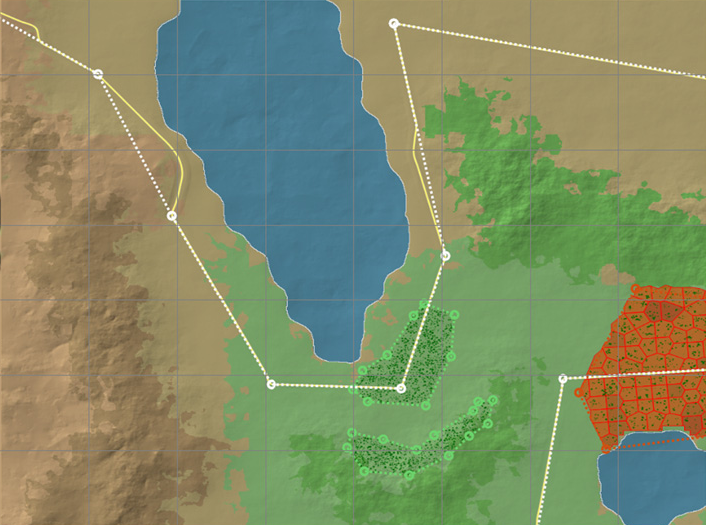
\includegraphics[height=6cm]{input_map.png}

      \tiny Image extracted from [STdKB11].
    \end{center}
  \end{figure}
\end{frame}

\begin{frame}{Environment Generation --- General Layout}
  \begin{figure}
    \begin{center}
      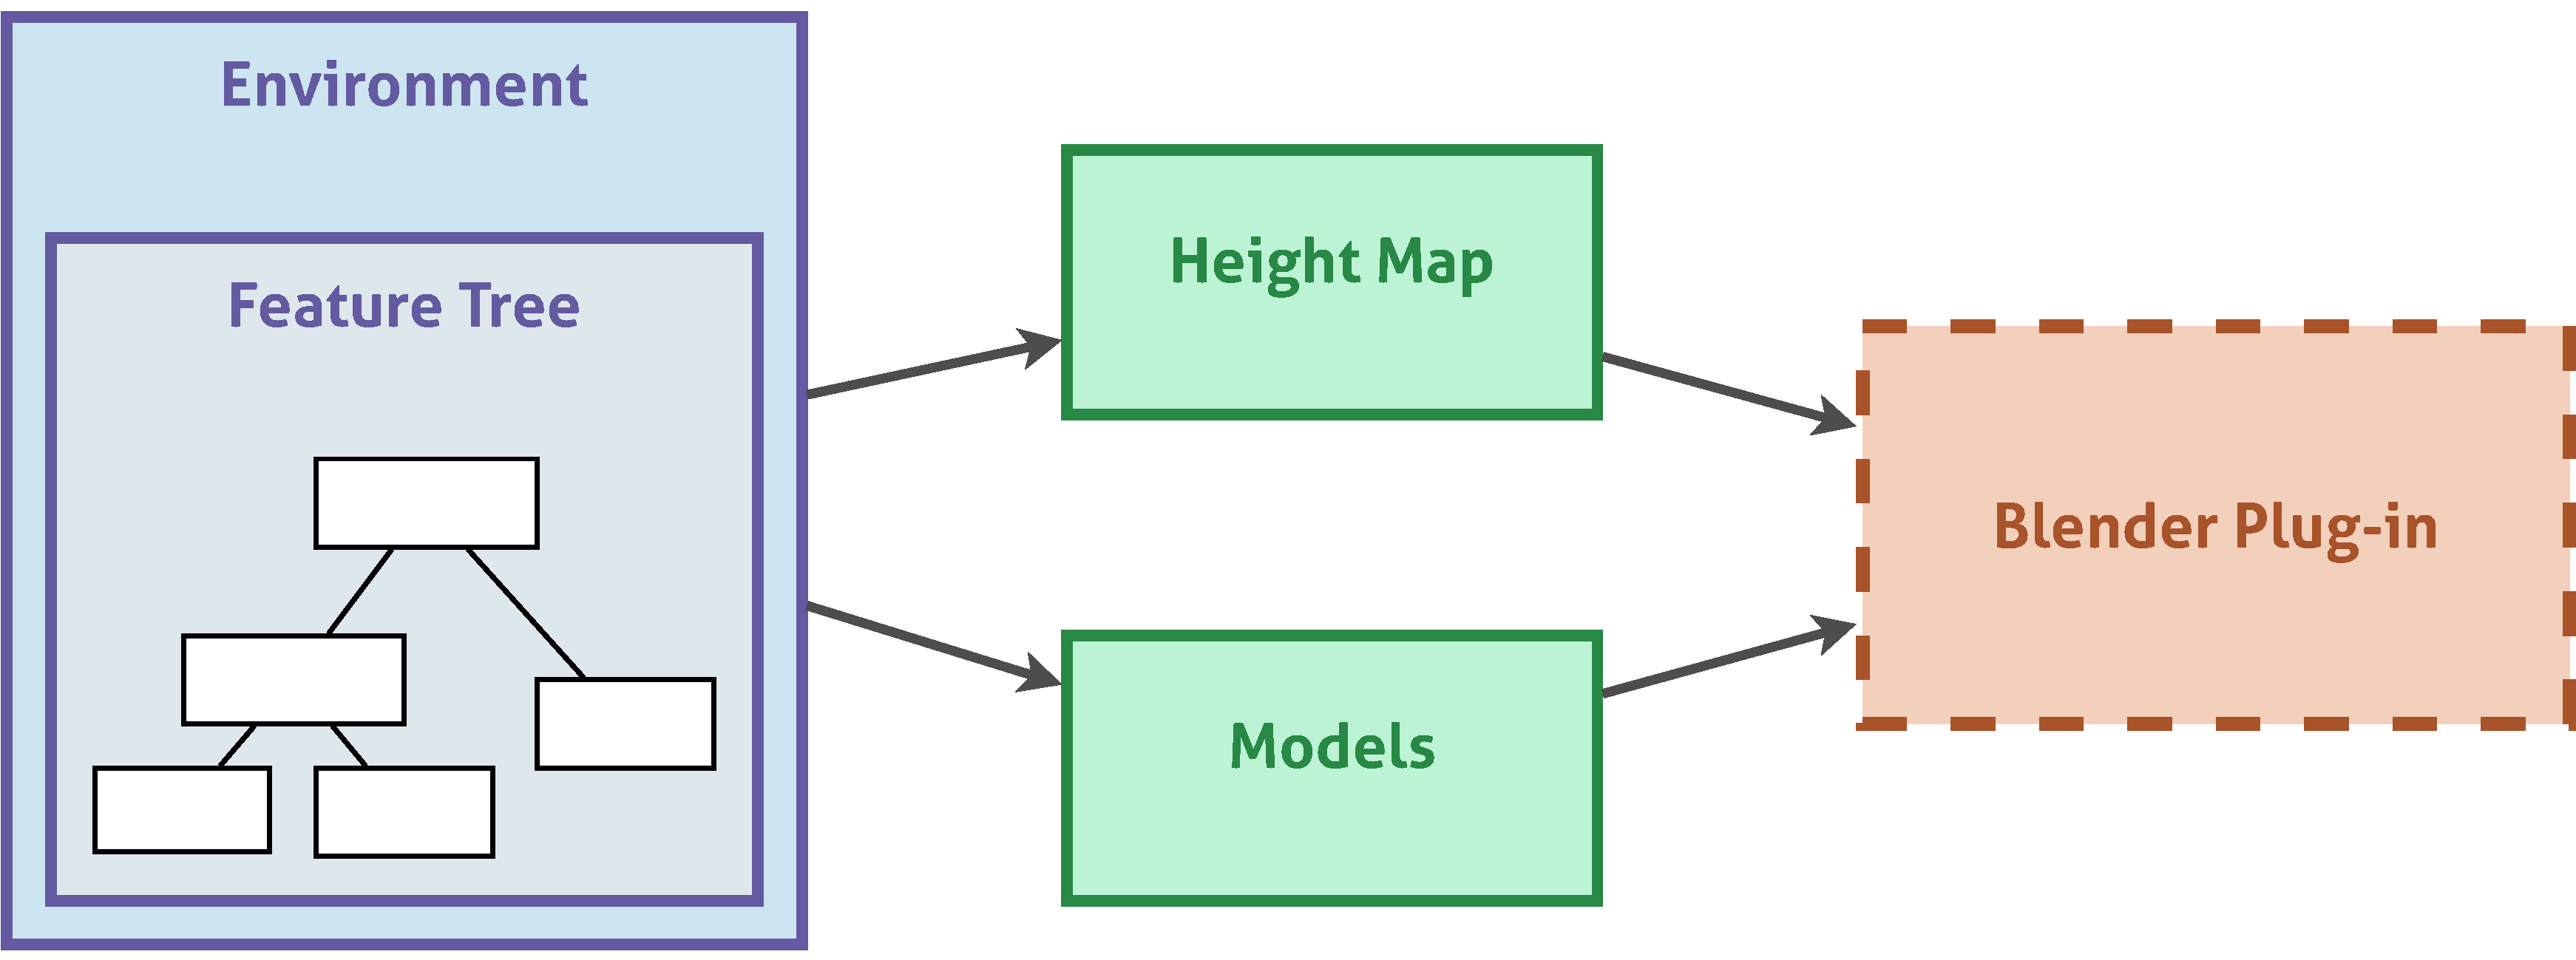
\includegraphics[width=10cm]{env_global.pdf}
    \end{center}
  \end{figure}
\end{frame}

\begin{frame}{Features}
  \begin{itemize}
    \item Forest
    \item Mountain
    \item Road
    \item Cities
    \item Water (river, lake)
    \item ...
  \end{itemize}
\end{frame}

\begin{frame}{Features}
  \begin{figure}
    \begin{center}
      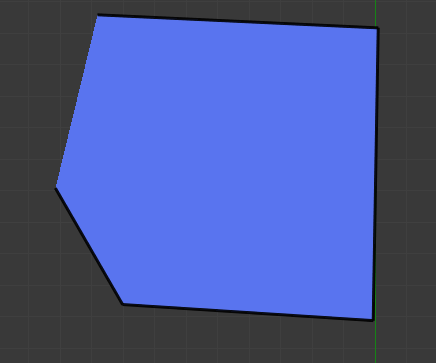
\includegraphics[width=4cm]{feature}
    \end{center}
  \end{figure}
  Feature:
  \begin{itemize}
    \item {\color{Cerulean}shape}
    \item \texttt{z(x,y)} : height function
    \item \texttt{models} : list of models
  \end{itemize}
\end{frame}

\begin{frame}{Feature Tree}
  \only<1>{
  \begin{figure}
    \begin{center}
      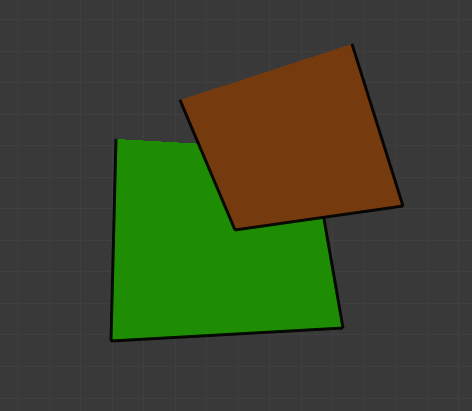
\includegraphics[width=4cm]{feature_2}
    \end{center}
  \end{figure}
  }
  
  \begin{figure}
    \begin{center}
      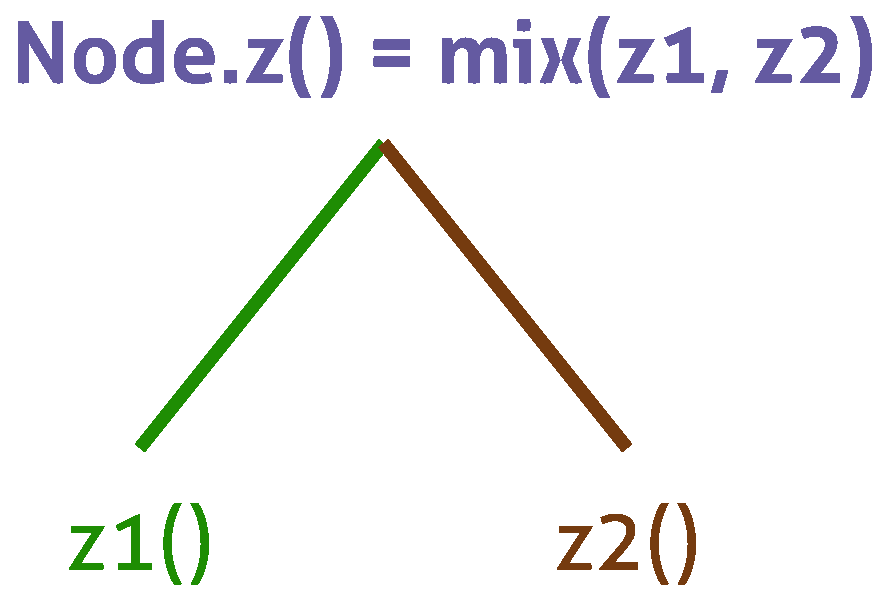
\includegraphics[width=5cm]{mix}
    \end{center}
  \end{figure}
  
  \only<2>{
  Depending on features, \texttt{mix(z1, z2)} could be:
  \begin{description}
    \item[Blend]:  Mean(z1(), z2())
    \item[Addition]: z1() + z2()
    \item[Replace]: Fixed to z1()
  \end{description}
  }
\end{frame}

\begin{frame}{Demo}
\end{frame}

\begin{frame}{What is missing}
  \begin{itemize}
    \item Live modifications
    \item City feature
  \end{itemize}
\end{frame}

\bgroup
\setbeamercolor{background canvas}{bg=black}
\begin{frame}[plain]{}
\end{frame}
\egroup

\begin{frame}{What is missing}
\begin{LARGE}
\begin{center}
  Thank you for your attention!
  
  Any questions?
    \end{center}
  \end{LARGE}
\end{frame}


\begin{frame}[allowframebreaks]{Bibliography}
  \begin{thebibliography}{10}

  %% original .bib  
  %%  @ARTICLE{cle,
  %% author = "liste-noms-auteur",
  %% title = "titre-article",
  %% journal = "nom-journal",
  %% year = "annee-parution",
  %% }
  %% becomes   
  %% \bibitem[label]{cle}
  %%   author
  %%   \newblock title
  %%   \newblock journal, issue, year

    %% Crowd
  \bibitem{GCCDLM2010}
    Guy S. J., Chhugani J., Curtis S., Dubey P., Lin M., Manocha~D.
    \newblock PLEdestrains: a least-effort approach to crowd simulation
    \newblock \emph{Proceedings of the 2010 ACM SIGGRAPH/Eurographics Symposiom on Computer Animation.} 2010

  \bibitem{VGLM2009}
    Van den Berg J., Guy S. J., Lin M., Manocha D.
    \newblock Reciprocal $n$-body collision avoidance
    \newblock \emph{Proc. Intl. Symposium on Robotics Research.} 2009

  \bibitem{MFCD2010}
    Multon F., France L., Cani M.-P., Debunne G.
    \newblock Computer Animation of Human Walking: a Survey
    \newblock \emph{Journal of Visualization and Computer Animation,} John Wiley \& Sons, 1999, 10, pp.39-54.


    %% Env
  \bibitem{STdKB11}
    Swelk R. M., Tunetel T., De Kraker K.J., Bidarra R.
    \newblock A declarative approach to procedural modeling of virtual worlds
    \newblock \emph{Computers \& Graphics} 35, 2 (2010), 352-363

  \bibitem{GGPGBGB15}
    Génevaux J.-D., Galin E., Peytavie A., Guérin E., Briquet C., Grosbellet F., Benes B.
    \newblock Terrain Modelling from Feature Primitive

  \bibitem{CEWMZ08}
    Chen G., Esch G., Worka P., Müller P., Zhang E.
    \newblock Interactive procedural street modeling
    \newblock \emph{ACM Transactions on Graphics (SIGGRAPH) 27}, 3 (2008), 103:1-103:10

% \bibitem{VKWHAM12}
%   Vanegas C.A., Kelly T., Weber B., Halatsch J., Allaga D., Müller P.
%   \newblock Procedural generation of parcels in urban modeling
%   \newblock \emph{Computer Graphics Forum: Proceedings of Eurographics 2012,} Eurographics Association, 2012

% \bibitem{GPMG10}
%   Galin E., Peytavie A., Maréchal N., Guérin E.
%   \newblock Procedural generation of roads
%   \newblock \emph{Computer Graphics Forum 29,} 2 (2010), 429-438

  %%  GCC10, MPB05, STdKB11, VKXW12

  \end{thebibliography} 
\end{frame}

\begin{frame}{Theme}
  Used the theme \emph{mtheme} by Matthias Vogelgesang, licensed under a Creative Commons
  Attribution-ShareAlike 4.0 International License.
\end{frame}

\end{document}
